\documentclass[11pt]{article}

\usepackage[margin=1in]{geometry}
\usepackage{amsmath,amssymb,amsthm,mathtools}
\usepackage{booktabs,tabularx,array}
\usepackage{graphicx}
\usepackage{caption}
\usepackage{float}
\usepackage{enumitem}
\usepackage{xcolor}
\usepackage[round]{natbib}
\usepackage[expansion=false]{microtype}
\usepackage{titlesec}

% Compact run-in headings within each numbered subsection.
\titleformat{\subsubsection}[runin]
  {\normalfont\normalsize\bfseries}{\thesubsubsection}{0.6em}{}
\titlespacing*{\subsubsection}{0pt}{0.6\baselineskip}{0.6em}
\usepackage{hyperref}

\graphicspath{{../figures/}{figures/}}
% Oct 9 build: policy numbers generated for the deck (\pol{case.field}).
% generated by build_prod_tables.py from output/model/reconciliation_14p40_20261007
\expandafter\def\csname pol:end_phi095.own_18_29_pp\endcsname{+26.12}
\expandafter\def\csname pol:end_phi095.own_18_29_pp.1\endcsname{+26.1}
\expandafter\def\csname pol:end_phi095.pop_pct\endcsname{-1.09}
\expandafter\def\csname pol:end_phi095.pop_pct.1\endcsname{-1.1}
\expandafter\def\csname pol:end_phi095.price_pct\endcsname{-0.73}
\expandafter\def\csname pol:end_phi095.price_pct.1\endcsname{-0.7}
\expandafter\def\csname pol:end_ptax2.own_18_29_pp\endcsname{+0.47}
\expandafter\def\csname pol:end_ptax2.own_18_29_pp.1\endcsname{+0.5}
\expandafter\def\csname pol:end_ptax2.pop_pct\endcsname{+0.68}
\expandafter\def\csname pol:end_ptax2.pop_pct.1\endcsname{+0.7}
\expandafter\def\csname pol:end_ptax2.price_pct\endcsname{-5.34}
\expandafter\def\csname pol:end_ptax2.price_pct.1\endcsname{-5.3}
\expandafter\def\csname pol:fp_baseline.births_pct\endcsname{+0.00}
\expandafter\def\csname pol:fp_baseline.births_pct.1\endcsname{+0.0}
\expandafter\def\csname pol:fp_baseline.own_18_29_pp\endcsname{+0.0}
\expandafter\def\csname pol:fp_baseline.own_18_29_pp.1\endcsname{+0.0}
\expandafter\def\csname pol:fp_baseline.price_pct\endcsname{+0.00}
\expandafter\def\csname pol:fp_baseline.price_pct.1\endcsname{+0.0}
\expandafter\def\csname pol:fp_phi095.births_pct\endcsname{-1.45}
\expandafter\def\csname pol:fp_phi095.births_pct.1\endcsname{-1.4}
\expandafter\def\csname pol:fp_phi095.own_18_29_pp\endcsname{+25.2}
\expandafter\def\csname pol:fp_phi095.own_18_29_pp.1\endcsname{+25.2}
\expandafter\def\csname pol:fp_phi095.price_pct\endcsname{+0.00}
\expandafter\def\csname pol:fp_phi095.price_pct.1\endcsname{+0.0}
\expandafter\def\csname pol:fp_phi100.births_pct\endcsname{-1.35}
\expandafter\def\csname pol:fp_phi100.births_pct.1\endcsname{-1.3}
\expandafter\def\csname pol:fp_phi100.own_18_29_pp\endcsname{+28.8}
\expandafter\def\csname pol:fp_phi100.own_18_29_pp.1\endcsname{+28.8}
\expandafter\def\csname pol:fp_phi100.price_pct\endcsname{+0.00}
\expandafter\def\csname pol:fp_phi100.price_pct.1\endcsname{+0.0}
\expandafter\def\csname pol:fp_price110.births_pct\endcsname{-4.90}
\expandafter\def\csname pol:fp_price110.births_pct.1\endcsname{-4.9}
\expandafter\def\csname pol:fp_price110.own_18_29_pp\endcsname{-2.8}
\expandafter\def\csname pol:fp_price110.own_18_29_pp.1\endcsname{-2.8}
\expandafter\def\csname pol:fp_price110.price_pct\endcsname{+10.00}
\expandafter\def\csname pol:fp_price110.price_pct.1\endcsname{+10.0}
\expandafter\def\csname pol:ge_phi100.births_pct\endcsname{-0.11}
\expandafter\def\csname pol:ge_phi100.births_pct.1\endcsname{-0.1}
\expandafter\def\csname pol:ge_phi100.own_18_29_pp\endcsname{+28.9}
\expandafter\def\csname pol:ge_phi100.own_18_29_pp.1\endcsname{+28.9}
\expandafter\def\csname pol:ge_phi100.price_pct\endcsname{-1.97}
\expandafter\def\csname pol:ge_phi100.price_pct.1\endcsname{-2.0}
\expandafter\def\csname pol:ptax2_fp.births_pct\endcsname{-2.92}
\expandafter\def\csname pol:ptax2_fp.births_pct.1\endcsname{-2.9}
\expandafter\def\csname pol:ptax2_fp.own_18_29_pp\endcsname{+0.2}
\expandafter\def\csname pol:ptax2_fp.own_18_29_pp.1\endcsname{+0.2}
\expandafter\def\csname pol:ptax2_fp.price_pct\endcsname{+0.00}
\expandafter\def\csname pol:ptax2_fp.price_pct.1\endcsname{+0.0}
\expandafter\def\csname pol:ptax2_ge_r2.births_pct\endcsname{+0.01}
\expandafter\def\csname pol:ptax2_ge_r2.births_pct.1\endcsname{+0.0}
\expandafter\def\csname pol:ptax2_ge_r2.own_18_29_pp\endcsname{+2.3}
\expandafter\def\csname pol:ptax2_ge_r2.own_18_29_pp.1\endcsname{+2.3}
\expandafter\def\csname pol:ptax2_ge_r2.price_pct\endcsname{-5.53}
\expandafter\def\csname pol:ptax2_ge_r2.price_pct.1\endcsname{-5.5}

\newcommand{\pol}[1]{\ifcsname pol:#1\endcsname\csname pol:#1\endcsname\else\errmessage{Missing policy number #1}\fi}
\hypersetup{
  colorlinks=true,
  linkcolor=blue!50!black,
  citecolor=blue!50!black,
  urlcolor=blue!50!black
}

\setlength{\parindent}{0em}
\setlength{\parskip}{0.45em}
\setlength{\emergencystretch}{3em}
\setlist[itemize]{leftmargin=1.3em,itemsep=0.12em,topsep=0.12em}
\setlist[enumerate]{leftmargin=1.45em,itemsep=0.12em,topsep=0.12em}
\allowdisplaybreaks

\newtheorem{proposition}{Proposition}
\newtheorem{lemma}{Lemma}
\newtheorem{corollary}{Corollary}
\theoremstyle{definition}
\newtheorem{definition}{Definition}
\newtheorem{assumption}{Assumption}
\newtheorem{remark}{Remark}

\newcommand{\dd}{\mathrm d}
\newcommand{\E}{\mathbb E}
\newcommand{\1}{\mathbf 1}

\title{Fertility and Housing Tenure Choice}
\author{Tommaso De Santo}
\date{}

\begin{document}

\maketitle
\begin{abstract}
\end{abstract}

\pagebreak
\section{Introduction}
\label{sec:introduction}

% Author text.

% October 9, 2026 build: same preamble and structure as the October 5 build,
% brought in line with the JMP deck of Oct 9 (latex/JMP_slides/JMP_slides.tex,
% 14.402 base). Agent draft.
\newcommand{\mocktodo}[1]{\textcolor{red}{[TODO: #1]}}
% ============================================================================
% October 9, 2026 build (agent draft). Copy of 02c_motivating_evidence.tex
% brought in line with the JMP deck of Oct 9 (latex/JMP_slides/JMP_slides.tex):
% the deck motivates the model with three channels (tenure segmentation,
% wealth and down payments, the intergenerational allocation of large homes)
% and no longer shows the CPS fertility-by-income table, so that subsection
% is cut here. The moving-reasons panels are the deck's appendix figures
% (JMP_slides/assets/mv_*_f_c_y_all.png, PSID, May event-study estimates).
% Register: Boar, Gorea and Midrigan, Section 2.
% ============================================================================
\providecommand{\mocktodo}[1]{\textcolor{red}{[TODO: #1]}}

\section{Motivating Evidence}
\label{sec:empirical-evidence}

This section documents three facts that shape the model. First, large homes
are mostly owned: the rental market offers few dwellings large enough for a
family with several children. Second, most large owner-occupied homes are held
by older households without children at home, while young families hold few.
Third, households enlarge their dwelling and move into ownership within a few
years of the first birth, and then move less. Together these facts describe
how a young family obtains space for children. It needs a larger home early
in adult life, when its savings are smallest, and the large homes are mostly
sold rather than rented and mostly held by an older generation. Space,
tenure and wealth are therefore linked at the moment fertility is decided.
None of the facts isolates an exogenous change in fertility, and I do not use
them to argue that housing costs lower fertility.
Appendix~\ref{app:empirical-data} describes the data.

\subsection{Large homes are owned}

Figure~\ref{fig:tenure-by-size} divides the homes of each size in the 2023
American Housing Survey (AHS) by tenure. Of the homes with four or more
bedrooms, 87 percent are owner-occupied and 9 percent are rented; of the homes
with at most one bedroom, 13 percent are owner-occupied and 74 percent are
rented. Measured in rooms, the unit used in the rest of the paper, 43.0
percent of owner-occupied homes have seven or more rooms, against 7.5 percent
of rented homes. The gap persists among families: in households with children,
owners occupy 6.8 rooms on average and renters 5.2. Nearly half of renter households
with children, 48.7 percent, live in homes with at most two bedrooms,
against 7.4 percent of owner households with children.
% [DATA] AHS 2023 ahs_children_space_mismatch.csv (code/data/ahs_supply_snapshot/
% output_ahs_family_unit_menu_national/). These shares describe the
homes households occupy, not the homes offered for rent. They show that, in
the existing stock, a family that wants a large dwelling typically buys one.
% [DATA] AHS 2023 national PUF; code/data/ahs_supply_snapshot/ (sandbox
% FIGURES.md maps the figure to its source).

\begin{figure}[t]
\centering
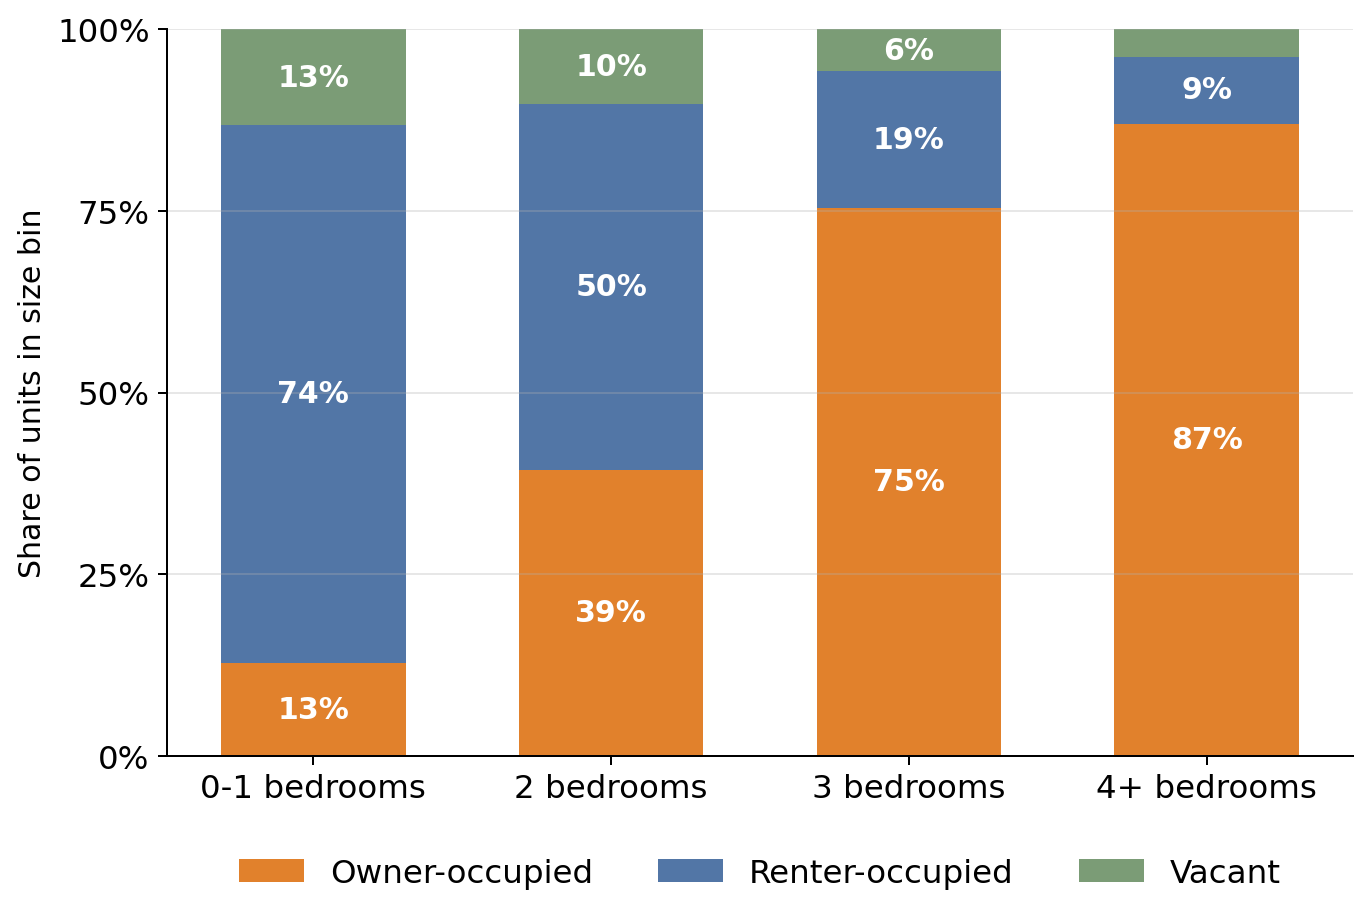
\includegraphics[width=0.62\linewidth]{ahs_tenure_share_within_size}
\caption{Tenure of the housing stock by number of bedrooms (AHS 2023)}
\label{fig:tenure-by-size}
\par\smallskip
\begin{minipage}{0.92\linewidth}
\footnotesize\textit{Notes:} Each bar divides the housing units with the
stated number of bedrooms into owner-occupied units, units rented for cash,
and vacant units. Units occupied without payment of cash rent and units whose
occupants have a usual residence elsewhere are excluded. Weighted by the
housing-unit weight. Source: American Housing Survey 2023, national
public-use file.
\end{minipage}
\end{figure}

\subsection{Who holds the large homes}

Most large owner-occupied homes are held by households without children at
home, and the largest group among them is old. Figure~\ref{fig:large-homes}
divides the owner-occupied homes with six or more rooms in 42 large
metropolitan areas in the 2023 American Community Survey (ACS) among six groups
of households, defined by the age of the householder and by whether a child of
the householder younger than 18 lives in the home. Households aged 60 to 85
without children at home hold 40.0 percent of these homes, and households
aged 40 to 59 without children at home another 21.8 percent. Households aged
22 to 39 with children hold 10.6 percent. Across all ages, 68.3 percent of the
large owner-occupied homes house no child of the householder, close to the
72.9 percent of all households in these areas without a child at home. What
the figure shows is therefore where the large homes sit by age, not that
childless households hold more than their share. I call the concentration of
large owner-occupied homes among older households the intergenerational
allocation of housing. The figure does not show that older households would
sell at some price, or that young families would have more children if they
held these homes.
% [DATA] ACS 2023 one-year, 42 metros, householders 22-85, 289,109 households;
% numbers as in the Oct 4 sandbox paper (reviewed there).
\mocktodo{name the builder of the large-homes figure in the data appendix
(not found in code/ by the Oct 4 sandbox review); the sandbox calls this
"intergenerational misallocation", which the title uses; choose the term.}

\begin{figure}[t]
\centering
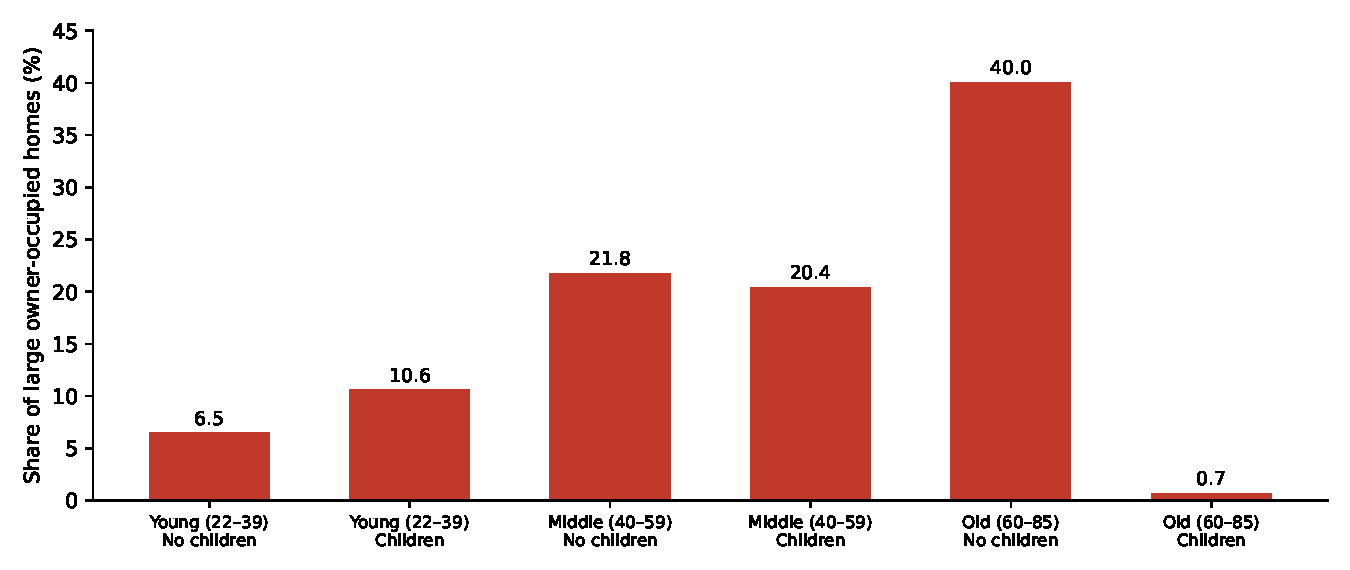
\includegraphics[width=0.9\linewidth]{large_homes_by_age_children_acs2023}
\caption{Who holds the large owner-occupied homes (ACS 2023)}
\label{fig:large-homes}
\par\smallskip
\begin{minipage}{0.92\linewidth}
\footnotesize\textit{Notes:} Each bar is the share of owner-occupied homes
with six or more rooms held by households in the group; the six shares sum to
100 percent. Groups are defined by the age of the householder and by whether
an own child of the householder younger than 18 lives in the household.
Householders aged 22 to 85 in 42 large metropolitan areas, weighted by the
household weight; 289,109 households.
\end{minipage}
\end{figure}

\subsection{Housing around the first birth}

The Panel Study of Income Dynamics (PSID) follows the same families from 1968
to 2019. I date each woman's first birth from her full history of biological
children and estimate event studies of her household's housing around it,
comparing first-time mothers with women who never have children, with the
estimator of Sun and Abraham (2021) and person and year
fixed effects. The reference window is two to three years before the birth,
so that moves made while expecting a child count as responses. The sample
keeps one woman per household and year who is its reference person or spouse.
% [DATA] mock 02_empirical_evidence.tex and data_appendix.tex; 63,338
% person-years, 3,655 first-time mothers, 1,654 childless women.

Households add about one room within four years of the first birth.
Figure~\ref{fig:emp-rooms-path} reports the path. The dwelling is 0.41 rooms
larger than in the reference window in the year of the birth, 0.82 rooms one
to two years later, and 1.03 rooms (standard error 0.07) three to four years
after it, on a base of 4.7 rooms. Fixing household position before the birth,
which removes a pre-trend that reflects who heads a household, the increase at
three to four years is 1.47 rooms (0.05). The added space comes with a move
into ownership, after which families move less (Figure~\ref{fig:emp-tenure-moves}).
The ownership rate is 11 percentage points higher in the birth window and 16
points higher three to four years later, on a base of 41 percent. The
probability of having moved since the previous interview falls by 16 to 21
points after the birth and stays lower for a decade, and among those who do
move, the share moving for more space doubles, from 12 to about 25 percent.
The ACS shows the same pattern at a point in time: among household heads aged
30 to 55, those whose oldest child is under four are 12.8 percentage points
more likely to own than heads without children.
% [DATA] ACS 2005-06 recent-parent gap 0.12761 (same as Section 4 target).

\begin{figure}[t]
\centering
\includegraphics[width=0.88\linewidth]{first_birth_rooms_psid}
\caption{Rooms around the first birth (PSID)}
\label{fig:emp-rooms-path}
\par\smallskip
\begin{minipage}{0.92\linewidth}
\footnotesize\textit{Notes:} Interaction-weighted event-study estimates in
two-year windows of event time, with 95 percent confidence intervals from
standard errors clustered by person. One woman per household-year who is the
reference person or spouse; 63,338 person-years, 3,655 first-time parents and
1,654 childless women. The hollow marker is the omitted reference window,
years $-3$ and $-2$. Mean rooms in the reference window: 4.70.
\end{minipage}
\end{figure}

\begin{figure}[t]
\centering
\includegraphics[width=0.92\linewidth]{first_birth_tenure_moves_psid}
\caption{Ownership and moving around the first birth (PSID)}
\label{fig:emp-tenure-moves}
\par\smallskip
\begin{minipage}{0.92\linewidth}
\footnotesize\textit{Notes:} Same sample, estimator and reference window as
Figure~\ref{fig:emp-rooms-path}. ``Moved for more space'' equals one if the
household moved since the previous interview and gave more space as the first
reason. Means in the reference window: ownership 0.41, moved 0.58.
\end{minipage}
\end{figure}

Figure~\ref{fig:emp-move-reasons} splits moves by the reason the household
gives. The annual probability of moving for more or better housing rises by
about 2.5 percentage points in the year before and the year of the birth and
returns to its earlier level within about five years. Moves for the
neighborhood, schools or proximity do not change around the birth. The
response to the first child is a demand for space, not for location.

\begin{figure}[t]
\centering
\begin{minipage}{0.48\linewidth}\centering
{\small Expansion or better housing}\par\smallskip
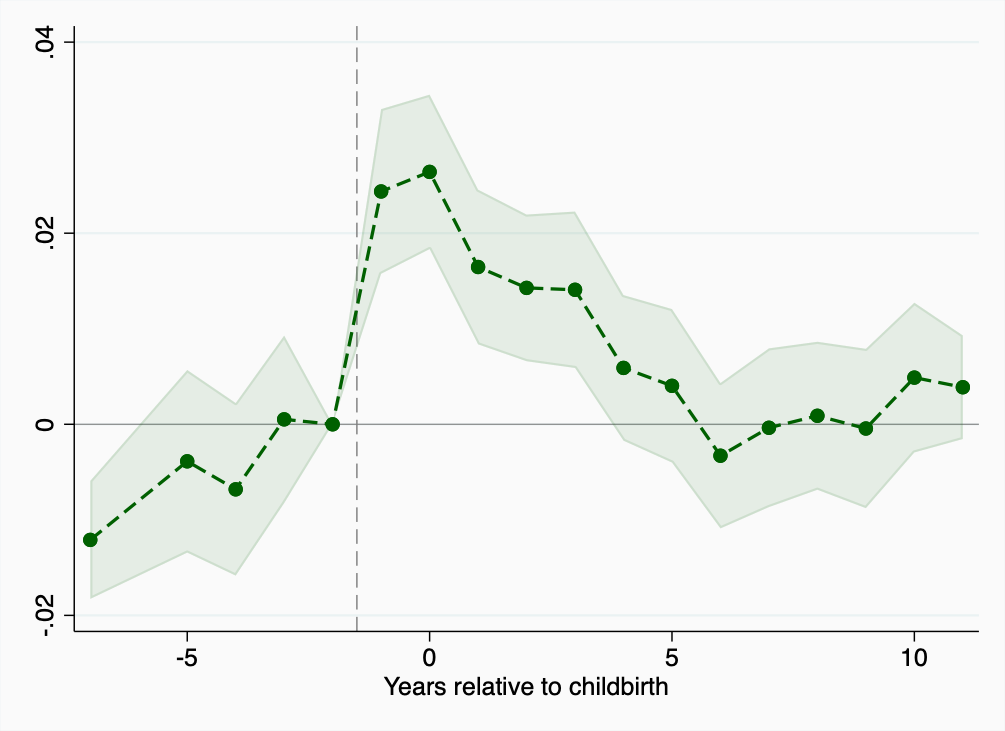
\includegraphics[width=\linewidth]{../JMP_slides/assets/mv_s_f_c_y_all.png}
\end{minipage}\hfill
\begin{minipage}{0.48\linewidth}\centering
{\small Neighborhood, schools, or proximity}\par\smallskip
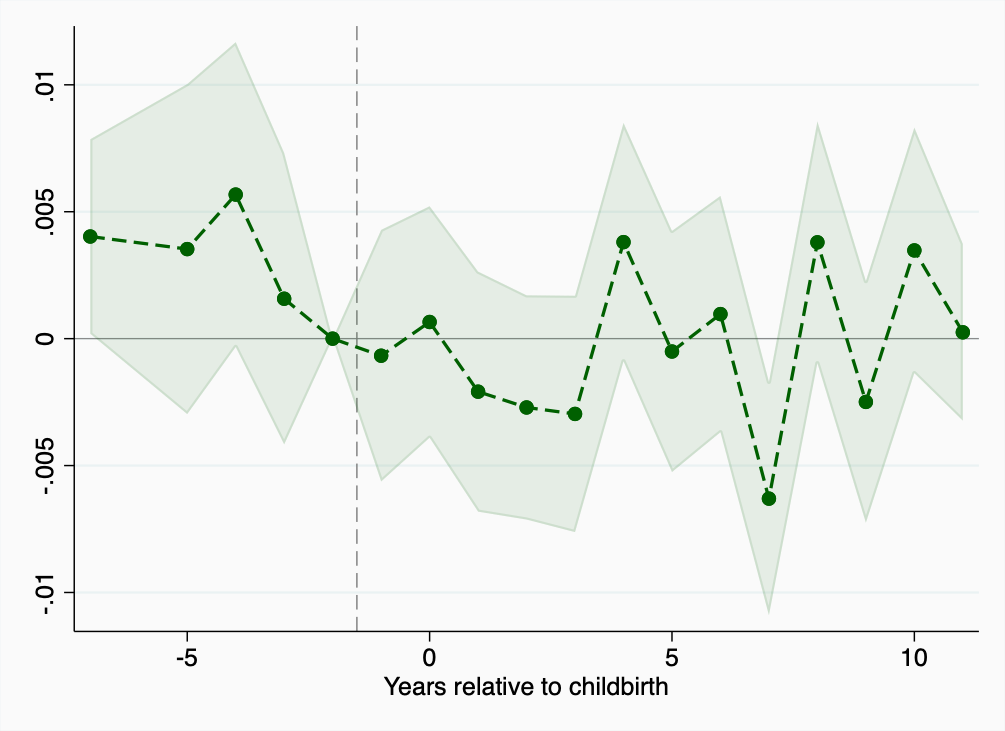
\includegraphics[width=\linewidth]{../JMP_slides/assets/mv_n_f_c_y_all.png}
\end{minipage}
\caption{Reasons for moving around the first birth (PSID)}
\label{fig:emp-move-reasons}
\par\smallskip
\begin{minipage}{0.92\linewidth}
\footnotesize\textit{Notes:} Event-study estimates of the probability of a move
for the stated reason, relative to the reference window, from the May
specification of the PSID event study.
\mocktodo{these are the deck's May estimates; the rooms and tenure figures
above are the September estimates. Re-estimate the reasons on the September
sample, or say in the notes that they come from the earlier specification.}
\end{minipage}
\end{figure}

\subsection{Implications for the model}

These facts motivate the three features that set the model apart from a
life-cycle model with a generic cost of children. Because children need
space and households add it around the first birth, fertility and housing
are chosen jointly, and a family needs a minimum of space before additional
rooms raise its welfare. Because large homes are mostly owned, the model
limits the size of rental units, so a family that wants a large home must buy
it; I call this tenure segmentation. Because buying requires a down payment,
paid out of wealth and current income, the wealth of young households and its
timing matter.
And because the large homes sit with older households, the price of space for
young families depends on the whole age distribution of households; the model
is an overlapping-generations economy in which one house price clears a
market shared by all ages.

% ============================================================================
% October 9, 2026 build (agent draft). Model section rewritten from
% 03b_model.tex in the notation of the JMP deck of Oct 9
% (latex/JMP_slides/JMP_slides.tex, frames "Environment" to "Equilibrium" and
% "Utility Specification"). Economic content is the engine of the 14.402
% base point (one-birth Estate A + net-estate floor, balanced property-tax
% rebate, PSID wealth-levels entry, post-interest transaction timing). The
% supply curve is written as in the deck, H = H0 P^eta, with H0 = 6.805: the
% engine writes H0_code (u P / r_bar)^eta with u the per-period user-cost
% rate and r_bar = 0.16, so H0 = H0_code (u / r_bar)^eta (commit feaacb00);
% the policy drivers rescale r_bar with u, so the curve in P is unchanged
% when the property tax changes.
% ============================================================================
\providecommand{\mocktodo}[1]{\textcolor{red}{[TODO: #1]}}

\section{Model}
\label{sec:model}

Motivated by these observations, I build a life-cycle model in which the same
households choose when to have children, how much housing to occupy, and
whether to rent or own it. Households live in an overlapping-generations
economy, face persistent earnings risk, and save in a single bond. Children
raise the household's needs for consumption and, above all, for space. Space
can be rented or bought. A room costs the same per period whether it is
rented or owned, but the largest dwellings are available only to owners,
owners enjoy their home somewhat more, selling a home is costly, and buying
one requires a down payment, which the household pays out of its wealth and
the income of the period. House prices and rents are determined in
equilibrium by an upward-sloping supply of housing. The government runs a pay-as-you-go pension system and taxes
property, and it returns the property-tax revenue to households as an equal
transfer.

\subsection{Environment}

Time is discrete and a period lasts four years. I describe the households,
their preferences, earnings, housing, the financial market and the
government in turn.

\subsubsection*{Demographics.}
A household enters the economy at age 18 and lives at most through age 85.
Let $a$ index its age, $a_R$ the age of retirement, 66, and $J$ the last age.
It works until $a_R$ and then receives a pension. From retirement on, it
survives from one period to the next with probability $s_a<1$; before
retirement $s_a=1$.
% [MODEL INPUT] ages 18,22,...,82 (17 cells), retirement at cell 12 (age 66),
% survival 0.9391, 0.9185, 0.8850, 0.8300 for cells 12-15, certain death after
% age 82.
\mocktodo{name the source of the survival probabilities (not documented in the
repository).}
Each household is one decision unit; I do not model the formation or
dissolution of couples.

Let $n_t$ denote the number of children ever born to the household and $m_t$
the number currently living at home. Births are possible from 18 through
age 45, at most one per period. Each child at home leaves independently with
probability $\lambda$ per period, so that a child stays on average
$1/\lambda$ periods; departure lowers $m_t$ but not $n_t$. I keep track of
$n_t$ up to three, with the last state standing for three or more. Children
are dependents: they do not work and do not make decisions.
% [MODEL INPUT] fertile cells ages 18-42 (decision at the start of each
% four-year period, so births up to age 45); lambda = 2/9 per period, mean stay
% 18 years; top state n = 3 = "3+".

\subsubsection*{Preferences.}
A household values consumption $c_t$, housing services $\hat h_t$, and
children at home. Its flow utility is
\begin{equation}
 u_t(c_t,\hat h_t;m_t)
 =\frac{1}{1-\sigma}\left(\frac{c_t^{\alpha_0}\,\hat h_t^{\,1-\alpha_0}}{e(m_t)}\right)^{1-\sigma}
 +v(m_t),\qquad v(m_t)=\psi_t\, m_t^{1-\gamma}.
 \label{eq:m-utility}
\end{equation}
The first term is utility from the consumption--housing composite per
equivalent adult. The equivalence scale
\begin{equation}
 e(m_t)=\left(\frac{2+\omega\, m_t}{2}\right)^{\nu}
 \label{eq:m-escale}
\end{equation}
measures how many adult equivalents the household contains relative to a
childless couple, so that the same spending buys less utility per person in a
larger family (as in Scholz, Seshadri and Khitatrakun, 2006); it depends on
the children at home, $m_t$, not on the children ever born. The second term,
$v(m_t)$, is the direct benefit of children at home, with $\psi_t>0$ its
level and $\gamma\in[0,1)$ the rate at which the benefit of an additional
child declines.
% [CODE] shared.py 290-312: c_bar = 0 under eqscale, escale =
% (((2+0.7 m)/2)^0.7)^(sigma-1) with m = children at home (cs), which is
% e(m)^(sigma-1), the multiplier that makes u(x/e) = e^(sigma-1) x^(1-sigma)/(1-sigma);
% child_preferences.py 31-33: benefit = psi_child m^(1-curvature) for m >= 1. The level $\psi_t$
carries a time subscript because it is the object that changes in the
historical exercise of Section~\ref{sec:quant-transition}. Becoming a parent
carries, in addition, a one-time utility cost $\xi$ at the first birth.

Children need room. A household with children at home obtains services only
from the space in excess of a minimum $\bar h(m_t)=h_P\,\1\{m_t>0\}$:
\begin{equation}
 \hat h_t=
 \begin{cases}
 h^R_t-\bar h(m_t), & \text{renter of } h^R_t \text{ rooms},\\[2pt]
 \chi\bigl[h_t-\bar h(m_t)\bigr], & \text{owner of } h_t \text{ rooms},
 \end{cases}
 \qquad \chi>1 .
 \label{eq:m-services}
\end{equation}
The parenthood space requirement $h_P$ is the space a family needs before
additional rooms add to its welfare. It is measured in rooms and does not
depend on the number of children, so it is the first child that creates the
need for space. The owner multiplier $\chi$ captures the additional services
an owner obtains from a dwelling of a given size, for example from the
ability to adapt it, and applies only to the rooms above the requirement. A
household with children in a dwelling of $h_P$ rooms or fewer obtains
essentially no housing services, so in practice parents occupy more than
$h_P$ rooms, whether they rent or own.
% [CODE] owner services chi*(h - h_P) (kernels.py 922-931: ht_c = hsv -
% owner_h_bar_scale*hbc, clamped at 1e-10 when h <= h_P, then times
% owner_service_premium; strict_hbar_feasibility is never passed, so the
% option is dominated, not infeasible). Renter: rent on h_P is paid first,
% dc = cbc + ri*hbc, and ht_unc = (1-al)*surplus/ri (kernels.py 726-729,
% 833-855). h_bar = hbar_first_child_jump + hbar_child_rooms*m (shared.py
% 291-296). The deck's "Utility Specification" frame writes
% chi[h - hbar(m)] + [h^R - hbar(m)] as one expression; read tenure by tenure,
% it is (eq:m-services).
Together, \eqref{eq:m-utility} and \eqref{eq:m-services} define what a child
costs. At given prices, a first child raises the spending needed to reach a
given utility in two ways: through the equivalence scale, which scales up all
spending, and through the space requirement, which must be paid at the rent
of a room before any housing yields services. The second part is paid every
period the child is at home, by renters and owners alike.

\subsubsection*{Fertility.}
At the start of each fertile period, a household chooses whether to try for a
child. An attempt succeeds with probability $\pi_a$, which declines with age,
and adds one child: $n_{t+1}=n_t+1$. The decision is subject to type-I
extreme-value taste shocks $\varepsilon^F_t$ with scale $\kappa_1$ when the
household is childless and $\kappa_C$ when it already has children, so that
childlessness and family size can respond differently to the same change in
incentives. After the outcome of the attempt is known, the household chooses
its housing and saving for the period. Housing can therefore adjust to a
birth within the same period, which matches the timing of the room response
in Section~\ref{sec:empirical-evidence}.
% [MODEL INPUT] pi_a = 1 - 0.02 exp(0.134 (age - 18)), zero from 45
% (parameters.py 21-45).
% [CODE] household.py 1000-1016: V = birth_count_menu(VI, n, m, pi_j,
% kappa_fert if n == 0 else kappa_fert_continuation, first_birth_fixed_cost,
% cap = 1), where VI is the housing/saving value after the birth outcome;
% birth_count.py 46-84: with cap 1 the menu is {wait, attempt} and the
% attempt value is pi*(VI[n+1,m+1] - xi*1{n=0}) + (1-pi)*VI[n,m], which is
% (eq:m-wait-attempt) and (eq:m-attempt).

\subsubsection*{Firms and earnings.}
Competitive firms produce with effective labor, $Y_t=A L_t$, where
$L_t=\int_{a<a_R} e_a z_t\,\dd G_t$ and $G_t$ is the distribution of
households over states, so the wage per efficiency unit is $w=A$, which I
normalize to one. Before retirement, a household of age $a$ earns, after the
payroll tax,
\begin{equation}
 y^d_t(a,z_t)=(1-\tau^w)\,w\,e_a\,z_t ,
 \label{eq:m-earnings}
\end{equation}
where $e_a$ is a deterministic age profile and $z_t$ an idiosyncratic labor
efficiency. Efficiency follows a first-order autoregressive process in logs,
\begin{equation}
 \log z_{t+1}=(1-\rho_z)\mu_z+\rho_z\log z_t+\epsilon_{t+1},\qquad
 \epsilon_{t+1}\sim N(0,\sigma_z^2),
 \label{eq:m-ar1}
\end{equation}
where $\mu_z$ normalizes mean efficiency to one. Earnings risk is the only
source of income uncertainty. From $a_R$ on, every retiree receives the same
pension $\varpi_t$.
% [MODEL INPUT] rho_z = 0.735, sigma_z = 0.484 per four-year period; nine
% states; pension flat.
% [CODE] e5f_social_security.py 40-41: income[:, :J_R] = (1-tax)*wage*profile,
% retirees receive the pension; shared.py 114-131: income_at_state = y*z before
% retirement, the flat pension after (retirement_income_z_scale = 0), plus the
% rebate at every age.
\mocktodo{name the data source of the age profile $e_a$ (not documented in
the files read).}

\subsubsection*{Housing and tenure.}
Housing is measured in rooms and trades at price $P_t$ per room. An owner
lives in a house of $h_t\in\mathcal H=\{2,4,6,8,10\}$ rooms. A renter rents
any $h^R_t\in[0,\bar h^R]$ rooms at rent $r_t$ per room, with
$\bar h^R<\max\mathcal H$, so the largest dwellings are reachable only
through ownership, as in the American Housing Survey facts of
Section~\ref{sec:empirical-evidence}. I call this tenure segmentation. Owners
pay depreciation $\delta_H$ and property tax $\tau^p_t$ on the value of their
home each period. Selling a home costs a fraction $\psi^s$ of its value;
buying costs nothing beyond the price. The tenure and dwelling choice is
subject to type-I extreme-value taste shocks $\varepsilon^H_t$ with scale
$\kappa_T$, one for each option: renting, keeping the current home, or buying
each size in $\mathcal H$.
% [CODE] household.py 194-206: hcost = P h, heq = (1-psi) P h, ocst =
% (delta + tau_H) P h, dp = (1-phi) P h, bmo = -phi P h; kernels.py 383-474
% (tenure_logit_kernel): options tn = 0 rent, tn >= 1 own size tn, with the
% stay value used when tn equals the current size.

\subsubsection*{Rents and housing supply.}
Competitive landlords own the rental stock. A landlord buys a room at $P_t$,
pays depreciation and property tax, rents it out at $r_t$, and sells it at
$P_{t+1}$. Landlords finance themselves at the household bond return $R_b$,
so zero profits require that rent equal the user cost of housing,
\begin{equation}
 r_t=(R_b+\delta_H+\tau^p_t)P_t-P_{t+1},
 \qquad\text{and in a steady state}\qquad
 r=(R_b-1+\delta_H+\tau^p)P .
 \label{eq:m-rent}
\end{equation}
Because rent equals the user cost and households and landlords borrow and
save at the same rate, a room costs the same per period whether it is rented
or owned. Tenure matters for the cost of a family through four features
only: the size limit on rentals $\bar h^R$, the owner multiplier $\chi$, the
cost of selling $\psi^s$, and the down payment described next. Along a
transition, \eqref{eq:m-rent} prices rent net of the expected capital gain,
so when the price is expected to recover, rent lies below the static user
cost.
% [CODE] steady state: inputs.py 159, user_cost_rate = (R_gross - 1) + delta
% + tau_H = 0.18028 per period; equilibrium.py 641, r = user_cost_rate * p.
% The dated rule along a transition is implemented in the transition runner,
% which is not in the engine files reviewed; it is stated as in the deck.

Housing is supplied by a competitive construction sector with a constant
elasticity with respect to the price,
\begin{equation}
 H^s_t=H_0\,P_t^{\eta},
 \label{eq:m-supply}
\end{equation}
where $H_0$ sets the scale of the stock and $\eta$ is the supply elasticity.
In the baseline, the stock is on this curve at every date: it adjusts to the
price within a period. Section~\ref{sec:policy-slow} replaces this with a
stock that adjusts slowly toward the same curve.
% [MODEL INPUT] eta = 0.63; H0 = 6.805 on this scale (engine: H0_code 6.312
% on the scale (u P / 0.16)^eta).
% [CODE] distribution.py 3213-3223 and 3256-3257, native_phase_b.py 97-99:
% supply = H0 * (user_cost_rate * p / r_bar) ** xi_supply, xi_supply = 0.63,
% r_bar = 0.16; demand = renter rooms + owner rooms. H0 = 6.312 *
% (0.18028/0.16)^0.63 = 6.805. inputs.py: eta_supply = 1.75 is an unused
% field; the elasticity in the law is xi_supply.

\subsubsection*{Saving and mortgages.}
Households save in a one-period bond $b_{t+1}$ with gross return $R_b$, fixed
in the world market; $b_{t+1}<0$ is mortgage debt. Borrowing must be secured
by a home: a renter cannot borrow, $b_{t+1}\geq0$. At origination, a buyer
must put down at least a fraction $1-\phi$ of the price,
\begin{equation}
 b_{t+1}\geq-\phi\,P_t h_t ,
 \label{eq:m-ltv}
\end{equation}
and afterwards the house is collateral for an owner who stays,
$b_{t+1}\geq\min\{b_t,-\phi P_t h_t\}$: a stayer pays the interest on its
mortgage and does not borrow more. An owner whose debt exceeds
$\phi P_t h_t$ after a fall in the price is therefore not forced to repay,
but cannot borrow more. The down payment is paid out of the wealth the
household brings into the period and the income it earns during it. With the
budget constraint below, \eqref{eq:m-ltv} makes a purchase feasible when
$R_b b_t+y^d_t+T_t\geq(1-\phi)P_t h_t$, so a household with little wealth
can buy out of a period's income, and there is no separate rule for how the
down payment is financed. Two further restrictions keep estates
nonnegative. From retirement on, when the household may die, its debt may not
exceed the sale value of its home net of the selling cost,
$b_{t+1}\geq-(1-\psi^s)P_t h_t$. An owner may sell and return to renting only
if the net proceeds repay the mortgage, $R_b b_t+(1-\psi^s)P_t h_{t-1}\geq0$.
Mortgages carry no amortization schedule and no limit on payments relative
to income.
% [CODE] renter floor: household.py 47-58 (unsecured_credit_limit = 0, so
% b' >= 0). Origination: household.py 205-206 (dp = (1-phi) P h, bmo =
% -phi P h), kernels.py 955-959 (total_floor = bf + unsecured_floor, with the
% unsecured part zero); phi = 0.80. Down payment from post-interest wealth
% plus income: household.py 926-931, dp_choice = (dp_arr - income)/R and
% bmo_purchase = (bmo - income)/R; kernels.py 433-445, a buyer from renting
% is infeasible if b < dp_choice or b - P h/R < bmo_purchase, both of which
% read R b + y >= (1-phi) P h (income includes the rebate, shared.py
% 114-131). Stayer: kernels.py 976-979, total_floor = max(min(b, -phi P h),
% due_death_floor); household.py 61-72. Net-estate floor: household.py
% 40-44, -(1-psi) P h when death_possible_at_age (household.py 33-38: last
% cell or survival < 1, so from the retirement cell on); kernels.py 980-983
% applied to buyers and stayers. Sale solvency: kernels.py 417-420, selling to
% rent is infeasible if R b + (1-psi) P h < 0 (require_owner_sale_solvency;
% credit.py 5-19). A seller who rebuys needs R b + (1-psi) P h_old + y >=
% (1-phi) P h_new (kernels.py 447-451). No amortization, no PTI
% (household.py 729-742 forbid them with native_purchase_income).

\subsubsection*{Budget constraint.}
Transactions in housing take place after interest accrues on the bond carried
into the period. A household that enters with $h_{t-1}$ owned rooms (zero for
a renter) and leaves with $h_t$ owned rooms and $h^R_t$ rented rooms faces
\begin{equation}
 c_t+b_{t+1}+r_t h_t^R+(\delta_H+\tau_t^p)P_t h_t
 =R_b b_t+y_t^d(a,z_t)+T_t-\1\{h_t\neq h_{t-1}\}\,P_t\bigl[h_t-(1-\psi^s)h_{t-1}\bigr],
 \label{eq:m-budget}
\end{equation}
where $y^d_t$ is earnings after the payroll tax or the pension and $T_t$ is
the lump-sum transfer from the government. A renter has $h_t=0$, an owner
$h^R_t=0$, and a household that keeps its home pays no transaction. The sale
proceeds and the purchase price are not compounded: a household that sells
and buys within a period carries only the difference into next period's
interest.
% [CODE] post-interest timing (author-adopted Oct 3): household.py 317,
% Rv = R b + y with y including the rebate; kernels.py 417 (sale to rent, b +
% (1-psi) P h/R), 433 (purchase, b - P h/R), 447 (sell and rebuy, b +
% ((1-psi) P h_old - P h_new)/R), so transactions are added to the bond after
% interest and carried into next period's interest only as a net amount.
% Owner cost (delta + tau_H) P h each period: household.py 200.

\subsubsection*{Bequests.}
A household that dies leaves its estate net of the selling cost,
$w^e_{t+1}=b_{t+1}+(1-\psi^s)P_t h_t$, and values it according to
\begin{equation}
 B(w^e_{t+1})=\theta_0\,\frac{(\theta_1+w^e_{t+1})^{1-\sigma}}{1-\sigma},
 \label{eq:m-bequest}
\end{equation}
where $\theta_0$ governs the strength of the bequest motive and $\theta_1$
the extent to which bequests are a luxury.%
\footnote{The estate enters $B$ as $\max\{w^e_{t+1},0\}$. Under the
borrowing constraints above it is nonnegative at every age at which death is
possible, so the truncation never binds.}
Estates are not received by other households; entrants' wealth is drawn from
the data instead, as described below.
% [CODE] Estate A: household.py 845-856, Vbq = bequest_utility_vec(b' + hv)
% with hv = (1-psi) P h (bequest_utility_net_active); household.py 1548-1582,
% b = max(b, 0), scale theta0*(1 + theta_n nk) with theta_n = 0, utility
% (theta1 + b)^(1-sigma)/(1-sigma), the zero-estate normalization only if
% normalize_bequest_utility (default False; the earlier footnote claiming the
% engine subtracts theta0 theta1^(1-sigma)/(1-sigma) could not be verified
% and was removed). No estate tax, estate_receiver = 'none'. Death branch:
% household.py 868-869 (last cell) and 879-881, Vnr = s*Vnr + (1-s)*Vbq.

\subsubsection*{Government.}
The government runs two programs, each with a balanced budget in every
period. The pension system pays every retiree the same pension $\varpi_t$,
financed by the payroll tax $\tau^w$ on earnings. The property tax raises
$\tau^p_t$ times the value of the entire housing stock, owned and rented:
owners pay it directly, and renters pay it through the rent, into which the
landlord passes it by \eqref{eq:m-rent}. Its revenue is returned to all
households, of every age and tenure, as an equal lump-sum transfer $T_t$, the
rebate.
% [CODE] shared.py 595-610: revenue = tau_H * price * (rental rooms + owner
% rooms); fiscal_closure.py 59-69: T*N = revenue - grants, equal lump sum at
% all ages (property_tax_rebate_closure = 'balanced'); shared.py 114-131 adds
% T to income at every age. Pension: e5f_stationary_paygo.py 47-62 solves the
% flat pension that balances the payroll tax given the exogenous age-income
% mass; e5f_social_security.py 50-96 certifies the balance (PAYGO_TOL 1e-6).

\subsubsection*{Entry.}
Households enter at age 18 as childless renters. Each entrant draws its
efficiency from the stationary distribution of $z$. Its wealth comes from the
distribution of net worth among childless renters aged 18 to 24 who head their
household in the PSID, 1984 to 2019, with negative net worth set to zero.
Dollar amounts are converted to model units with one common scale, chosen so
that mean income in this sample equals mean earnings of entrants in the
model, and observations are assigned to efficiency states by income rank, so
that the poorest entrants in the data become the least productive entrants in
the model. The children born in the model form the entering households: the
number of entrants in each period equals the number of children born sixteen
and twenty years earlier, half from each cohort, divided by 2.1, so that the
population is constant when each household has 2.1 children on average.
% [CODE] adult_entry.py 14-32: entry = adjusted births / 2.1, where a birth
% into the top state n = 3 counts tfr_top_bin_weight = 3.602 children;
% native_phase_b.py 265-270 and distribution.py 1446-1457: split queue, half
% due 16 years after birth (4 periods) and half 20 (5 periods).
% distribution.py 597-613: entrants are childless renters at the first cell,
% z drawn from z_weights, wealth from the PSID law. entry_wealth.py 197-293:
% levels_rank law, negative net worth censored at zero, one scale lambda =
% model mean annual gross entry earnings (transfers excluded) / weighted mean
% sample family income, exact weighted income-rank allocation to z states.

\subsection{The household's problem}
\label{sec:m-household}

The state of a household at the start of a period is its age $a$, bond
position $b_t$, housing $h_{t-1}$, efficiency $z_t$, and children $n_t$ and
$m_t$. A period has two stages. The household first sees its fertility taste
shocks and decides whether to attempt a birth. It then learns whether the
attempt succeeded, sees its tenure taste shocks, and chooses tenure,
dwelling, consumption and saving. Children leave home and efficiency is drawn
between periods.

\subsubsection*{Housing and saving.}
After the birth outcome, the value of the household is
\begin{multline}
 V^H_t(b_t,h_{t-1},z_t,a,n,m)
 =\E_{\varepsilon_t^H}\max_{h_t,h_t^R,b_{t+1}}
 \Bigl\{u_t\big(c_t,\hat h_t;m\big)+\varepsilon_t^H(h_t)\\
 +\beta\,\E_t\Bigl[s_a V_{t+1}(b_{t+1},h_t,z_{t+1},a+1,n,m_{t+1})
 +(1-s_a)B(w^e_{t+1})\Bigr]\Bigr\}
 \label{eq:m-vh}
\end{multline}
subject to the budget constraint \eqref{eq:m-budget}, the services
\eqref{eq:m-services}, and the borrowing constraints: $b_{t+1}\geq-\phi
P_th_t$ for a household that buys or rents, $b_{t+1}\geq\min\{b_t,-\phi
P_th_t\}$ for an owner who stays, and, when death is possible,
$b_{t+1}\geq-(1-\psi^s)P_th_t$. The expectation is over next period's
efficiency $z_{t+1}$ and the number of children $m_{t+1}$ still at home. An
option is available only if it leaves room for a saving choice that
satisfies the borrowing constraints, and a sale only if the net proceeds
repay the mortgage. Given the option $o$ (renting, keeping
the home, or buying each size), let $V^o_t$ denote the value of the best
choice of $c_t$, $h^R_t$ and $b_{t+1}$. With the extreme-value shocks,
\begin{equation}
 V^H_t=\kappa_T\log\sum_{o}\exp\bigl(V^o_t/\kappa_T\bigr),
 \qquad
 \pi^H_{t,a}(o)=\frac{\exp(V^o_t/\kappa_T)}{\sum_{o'}\exp(V^{o'}_t/\kappa_T)} .
 \label{eq:m-tenure}
\end{equation}
Because the composite in \eqref{eq:m-utility} is Cobb--Douglas, a renter not
at the size limit spends a share $1-\alpha_0$ of its outlay net of the space
requirement on rooms above $h_P$.
% [CODE] kernels.py 383-474 (tenure_logit_kernel): VH = best_v +
% kappa*log(sum exp((V^o - best_v)/kappa)) over the feasible options, which is
% (eq:m-tenure); kernels.py 833-855: renter ht_unc = (1-al)*surplus/ri, capped
% at hR_max - h_bar.

\subsubsection*{Fertility.}
Before the birth outcome, a household with $n_t<3$ in a fertile period
compares waiting and attempting, with values
\begin{equation}
\begin{aligned}
 W_t^0&=V^H_t(b_t,h_{t-1},z_t,a,n_t,m_t),\\
 W_t^A&=\pi_a\Bigl[V^H_t(b_t,h_{t-1},z_t,a,n_t+1,m_t+1)-\xi\,\1\{n_t=0\}\Bigr]
 +(1-\pi_a)\,V^H_t(b_t,h_{t-1},z_t,a,n_t,m_t).
\end{aligned}
 \label{eq:m-wait-attempt}
\end{equation}
With scale $\kappa(n_t)=\kappa_1$ if $n_t=0$ and $\kappa_C$ otherwise, the
value at the start of the period is
\begin{equation}
 V_t(b_t,h_{t-1},z_t,a,n_t,m_t)
 =\E_{\varepsilon_t^F}\max\bigl\{W_t^0+\varepsilon^F_{t,0},\;W_t^A+\varepsilon^F_{t,A}\bigr\},
 \label{eq:m-fertility}
\end{equation}
and the probability of attempting a birth is
\begin{equation}
 \pi^F_{t,a}(b_t,h_{t-1},z_t,n_t,m_t)
 =\frac{\exp\{W_t^A/\kappa(n_t)\}}{\exp\{W_t^A/\kappa(n_t)\}+\exp\{W_t^0/\kappa(n_t)\}} .
 \label{eq:m-attempt}
\end{equation}
Outside the fertile ages, or with $n_t=3$, $V_t=V^H_t$. A birth is therefore
attempted when the value of the household with one more child, net of the
cost of becoming a parent, exceeds the value of waiting by enough to overcome
the taste shocks. Anything that changes the resources a household can devote
to the space a child requires, or the risk around them, changes the gap
$W^A_t-W^0_t$ and with it the probability of a birth.

\subsection{Equilibrium}
\label{sec:m-equilibrium}

Let $G_t$ be the distribution of households over states and $N_t$ the number
of households. Given parameters, an initial population $N_0$ and an initial
distribution $G_0$, an equilibrium is a sequence
$\{V_t,g_t,G_t,N_t,P_t,r_t,T_t,\varpi_t\}_{t\geq0}$ such that, at every date:
\begin{enumerate}
\item \emph{Households.} Given $\{P_{t'},r_{t'},T_{t'},\varpi_{t'}\}_{t'\geq
t}$, $V_t$ solves the household problem of Section~\ref{sec:m-household}
with continuation $V_{t+1}$, and the policy functions $g_t$ (fertility,
tenure, dwelling, consumption and saving) attain it.
\item \emph{Rents.} The rent satisfies the landlord's zero-profit condition
\eqref{eq:m-rent}.
\item \emph{Housing market.} The rooms occupied by owners and renters equal
the supply \eqref{eq:m-supply},
\[
 N_t\int\bigl[h_t+h^R_t\bigr]\dd G_t=H_0\,P_t^{\eta}.
\]
\item \emph{Government.} The pension system balances,
$\tau^w w\int_{a<a_R}e_az_t\,\dd G_t=\varpi_t\int_{a\geq a_R}\dd G_t$, and the
rebate returns the property-tax revenue,
$T_t=\tau^p_tP_t\int\bigl[h_t+h^R_t\bigr]\dd G_t$.
\item \emph{Population.} Births are $N_t\int\pi_a\pi^F_{t,a}\,\dd G_t$.
Households survive to the next age with probability $s_a$, and the children
born form new households when they reach adulthood, as described under Entry.
\item \emph{Consistency.} $G_{t+1}$ and $N_{t+1}$ follow from $G_t$ and $N_t$
under $g_t$, the shocks, survival, the departure of children and entry.
\end{enumerate}
A stationary equilibrium is an equilibrium in which prices, the pension, the
rebate and $G_t$ are constant. In a stationary equilibrium the population is
constant only if households have 2.1 children on average, so the house price
is the one at which the population reproduces itself, and the population is
the one that clears the housing market at that price. Two features of the
equilibrium are worth stating. First, the price of housing links fertility to
housing supply: more births raise the demand for rooms by families, which
raises $P_t$ and $r_t$ and with them the cost of the space a child requires.
Second, because the housing stock is durable and the population responds to
fertility only with a lag of a generation, a change in fertility moves the
price of space for decades.%
\footnote{In the calibration I normalize the 2007 population to one and set
$H_0$ so that the market clears at the price consistent with replacement. In
every counterfactual $H_0$ is held fixed and the population adjusts.}
% [CODE] production/README.md: price root = birth-renewal residual; H0
% derived under population_one, held fixed (fixed_h0) in counterfactuals.
% equilibrium.py (model) 84-96: renewal_root = adjusted_births/(2.1*entry)
% - 1, implied H0 = demand/(u P/r_bar)^xi; native_phase_b.py 25-26, 126-127:
% RENEWAL_TOL 1e-6, population = supply/demand under fixed_h0;
% distribution.py 1101-1102 (survival), 1219-1264 (child departure via
% Pi_child and entrants maturing), 1419-1430 (property-tax revenue and rebate
% outlays on the current distribution).

\subsection{A graphical illustration}
\label{sec:m-illustration}

Figure~\ref{fig:m-illustration} summarizes how the equilibrium responds to a
fall in the preference for children. Summarize housing costs by $p$ and
fertility by $n(p;\psi)$, decreasing in $p$. Panel~(a) of the top row shows
the housing market: given the adult population $S$, the housing cost
$P(S;\psi)$ clears the market. Panel~(b) shows fertility as a function of the
housing cost. At $A$, housing clears at $(S_0,p_0)$ and fertility is at the
replacement rate $\bar n$. A fall in the preference from $\psi_0$ to $\psi_1$
first lowers fertility at the unchanged housing cost, from $A$ to $A'$
(middle row). With fewer children at home, housing demand falls and the
housing cost adjusts at the inherited population $S_0$, from $A'$ to $B$.
Over the following generations, smaller entering cohorts reduce housing
demand further (bottom row). Lower housing costs partly offset the decline in
the preference, and $C$ marks the new stationary outcome, at which fertility
is again at replacement with a smaller population and cheaper housing. The
quantitative transition of Section~\ref{sec:quant-transition} follows these
steps.

\begin{figure}[p]
\centering
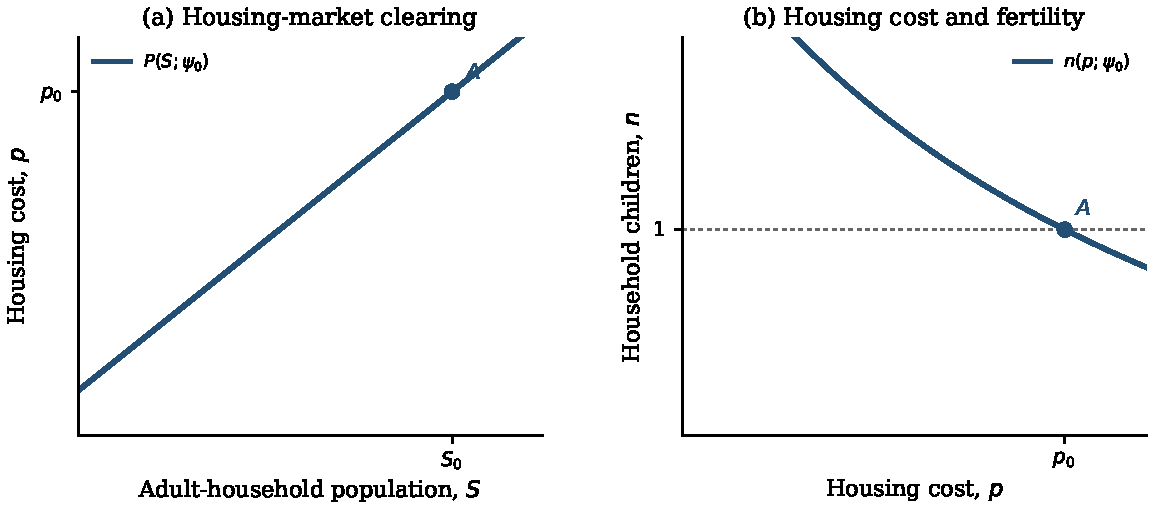
\includegraphics[width=0.86\linewidth]{september_housing_fertility_stage_initial}\\[0.4em]
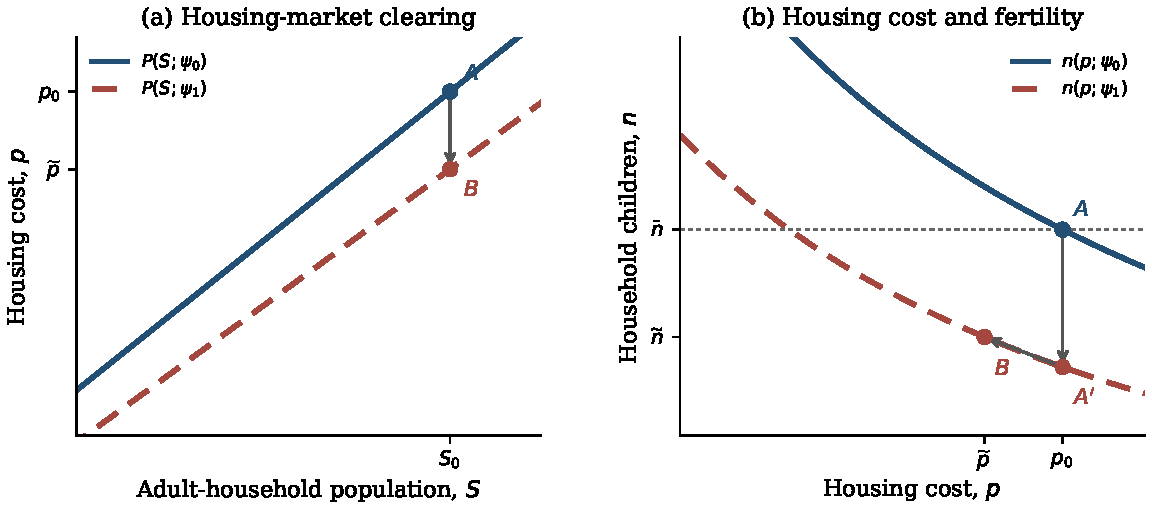
\includegraphics[width=0.86\linewidth]{september_housing_fertility_stage_impact}\\[0.4em]
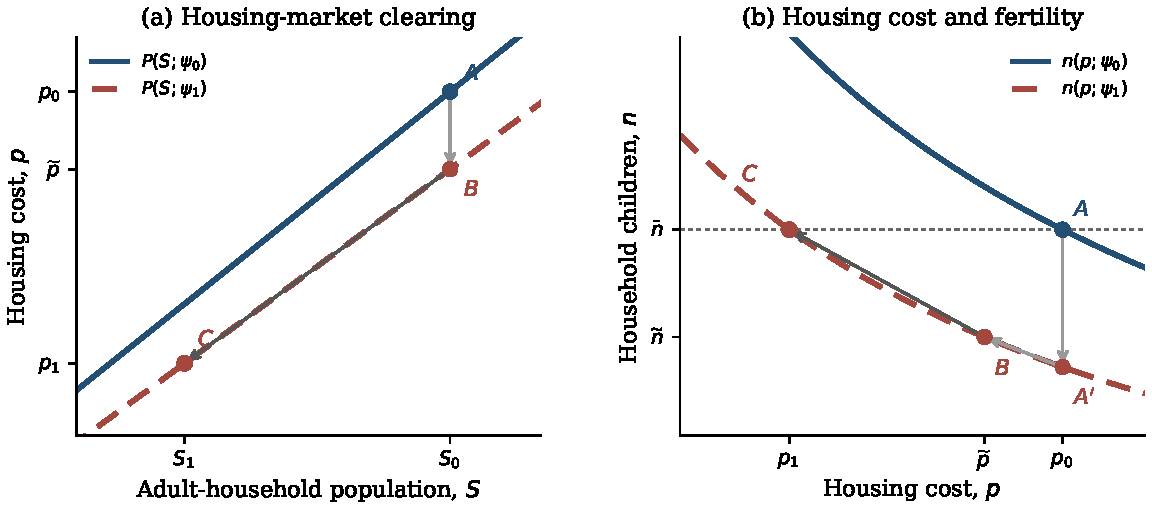
\includegraphics[width=0.86\linewidth]{september_housing_fertility_stage_adjustment}
\caption{Fertility, housing costs and population: initial steady state,
impact, and demographic adjustment}
\label{fig:m-illustration}
\par\smallskip
\begin{minipage}{0.92\linewidth}
\footnotesize\textit{Notes:} Schematic. Panel (a) of each row: housing-market
clearing; panel (b): housing cost and fertility. Top: the initial steady
state $A$. Middle: a fall from $\psi_0$ to $\psi_1$ ($A\to A'\to B$). Bottom:
demographic adjustment to the new stationary outcome $C$.
\end{minipage}
\end{figure}

% ============================================================================
% October 9, 2026 build (agent draft). Adapted from 04b_quantification.tex
% (Oct 6, base 15.07) to the 14.402 base point of the JMP deck of Oct 9.
% Fit, parameters and external inputs: latex/JMP_slides/prod_tables/
% (fit_full.tex, params.tex, external.tex; build_prod_tables.py, reading
% output/model/production/2007, promoted Oct 7: Mac round 3, chain 0, case
% 0010_nm, loss 14.402423836558775, selected_numerically_verified; receipt
% output/model/production/2007/PROMOTION_RECEIPT_20261007_mac_r3_chain0.md).
% Transition: H100 two-shock path, pair psi 0.1311 / 0.110
% (path_table_0.1311_0.110.md; figures
% output/model/jmp_slides_transition_figures_20261009/). 2023 table: deck frame
% "2023 Data and Model" (moments_2023_full_base14402.csv).
% ============================================================================
\providecommand{\mocktodo}[1]{\textcolor{red}{[TODO: #1]}}

\section{Quantification}
\label{sec:quant}

I treat the United States as an economy in transition to a smaller
population. The quantification has three steps. First, I calibrate a
stationary economy representing 2007, before the subsequent decline in
fertility, to match fertility, housing and wealth moments. Second, I hold
those parameters fixed and estimate a sequence of fertility shocks: two
unanticipated changes in the preference for children $\psi_t$ that match the
period fertility rate through 2023, carrying households and population
forward between the shocks. Third, I treat 2023 as a point on this
transition and project the economy forward, holding the preference for
children fixed after 2023. The policy experiments of
Section~\ref{sec:policy} all start from the same 2023 economy.

I organize the parameters into two groups. The first is set outside the
estimation, from external evidence or direct measurement. The second is
estimated by matching model moments to their empirical counterparts. I first
describe the data behind the targets and explain how annual data map into the
model's four-year period, because almost every parameter and moment passes
through that mapping.

\subsection{Data}
\label{sec:quant-data}

The targets combine five data sets, each chosen for the object it measures
best. Table~\ref{tab:quant-fit} lists every moment with its source. Fertility
moments come from the 2004 and 2006 CPS and the 2003--2006 natality records,
housing moments from the 2005--2006 ACS, the 2007 AHS and the PSID, and
wealth from the 2005 and 2007 PSID and the 2007 SCF.

\paragraph{Fertility.} The June Fertility Supplement of the CPS records the
number of children ever born to each woman. I pool the 2004 and 2006
supplements and measure childlessness and the share of mothers with exactly
one child among women aged 40 to 44, and the mean number of children ever born
among women aged 25. Children ever born are capped at three, the largest
number the model distinguishes. The timing of first births comes from the
NCHS natality files, which record every birth with the mother's age and the
birth order; I pool first births in 2003 to 2006.

\paragraph{Housing.} Mean rooms come from the 2007 AHS, for household heads
aged 18 to 85, without top-coding. Ownership among household heads aged 30 to
55 and the ownership gap between recent parents, whose oldest child is under
four, and heads without children come from the 2005--2006 ACS.
\mocktodo{state the dwelling-structure restriction used in both ACS ownership
moments (UNITSSTR codes 3--10 in the builder) and whether the model imposes it.}
The room response to the first birth is the PSID event-study estimate of
Section~\ref{sec:empirical-evidence} in the sample that fixes household
position before the birth: 1.465 rooms three to four years after the birth
(standard error 0.050). I use this sample rather than the household sample of
Figure~\ref{fig:emp-rooms-path}, which gives 1.03, because the model follows
the same households before and after the birth.

\paragraph{Wealth.} Aggregate net worth relative to aggregate annual gross
labor earnings comes from the 2005 and 2007 PSID: net worth of all household
heads aged 18 to 85, excluding business and farm equity and other real
estate, over gross labor earnings of heads aged 18 to 65. The bequest flow is
the annual flow of estates directed to children relative to aggregate net
worth in the 2007 Survey of Consumer Finances.

\subsection{From annual data to four-year periods}
\label{sec:quant-period}

A model period lasts four years. The unit of account is mean annual gross
labor earnings of working-age households, so a model value of one corresponds
to \$82,882 in the 2005 and 2007 PSID (2022 dollars). The mapping follows
three rules.

\paragraph{Stocks are measured in annual units; flows are four years long.}
Wealth, house prices and the bequest shifter $\theta_1$ are stocks and are not
rescaled. Income, consumption, rent and every other flow accrue over the whole
period, so a flow in the model is four times its annual counterpart. For
example, an entrant at age 18 with average efficiency earns
$4\times(1-0.080)\times0.721=2.65$ per period after the payroll tax, which is
0.72 times mean annual gross earnings. A moment that relates a stock to a flow
is computed against the annual flow, as in the data: the wealth target
divides net worth by annual gross earnings, and the bequest target divides the
estate flow over a period by four before dividing it by aggregate wealth.

\paragraph{Rates compound; hazards come from durations.}
Interest, discounting and depreciation compound over the four years. The gross
return is $R_b=1.02^4=1.082$, the period discount factor is
$\beta=\beta_{\text{ann}}^4$, and the period depreciation rate is
$1-(1-\delta_{\text{ann}})^4$. With $\beta_{\text{ann}}=0.940$, the period
discount factor is $0.781$. The property tax is the exception: it is a tax on
value levied each year, and I set the period rate to four times the annual
rate.%
\footnote{Compounding instead would give a period rate of 4.17 rather than
4.24 percent of value.}
Probabilities of events are period probabilities. Children leave home after
18 years on average, which I implement as a constant departure probability of
$\lambda=1/4.5=2/9$ per period for each child. Survival probabilities are
four-year probabilities between successive age cells. The probability $\pi_a$
that an attempt to have a child succeeds is the probability of a conception
within four years at that age.
\mocktodo{cite the source of the four-year conception probabilities and the
life table behind the survival probabilities.}
The earnings process is estimated directly at the four-year frequency rather
than converted from an annual process. I take non-overlapping four-year means
of household gross labor earnings in the annual PSID waves of 1984--1997,
remove age and year effects, and estimate $\rho_z=0.735$ from the first two
autocovariances of their logarithm. The implied annual persistence is
$0.735^{1/4}=0.926$.

\paragraph{Age-specific moments use the overlap of data ages with model cells.}
A model household of age $a$ occupies a four-year cell. A data statistic for
an age window weights each cell by the fraction of the cell that falls in the
window. Within a cell, a household's number of children is interpolated
linearly between its value at the start and at the end of the cell, which is
exact if births are spread uniformly over the four years. Women aged 40 to 44,
for example, overlap the cell $[38,42)$ for half its length and the cell
$[42,46)$ for three-quarters of its length, and children ever born at age 25
are read from the cell $[22,26)$, seven-eighths of the way from its start to
its end. For the mean age at first birth, I date a first birth in the model at
the midpoint of its cell and group the natality data into the same four-year
cells, so that both sides use the same representative ages.

The room response to the first birth is the one moment for which the period
length bounds how closely the model can mimic the data. In the model, I
compare households that have a first birth with otherwise identical
households that do not, one period, or four years, after the birth. The data
compare years three and four after the birth with years two and three before
it. The model's contrast is therefore a four-year response with no
pre-period, while the data's spans about six years.

\subsection{Parameters set outside the estimation}

Table~\ref{tab:quant-assigned} summarizes the parameters assigned outside the
estimation.

\paragraph{Demographics and preferences.}
Households enter at age 18, retire at 66, and live at most through age 85.
Survival is certain before retirement. Children remain at home for 18 years
on average. Births are possible through age 45, with the success probability
of an attempt falling from 0.98 at 18 to 0.50 at 42. I set risk aversion to
$\sigma=2$ and use the power equivalence scale of Scholz, Seshadri and Khitatrakun (2006) with
child weight $\omega=0.7$ and exponent $\nu=0.7$. The consumption weight
$\alpha_0=0.733$ is the expenditure share of nonhousing consumption among
childless renters in the 2019--2023 CEX. A birth into the state of three or
more children counts as 3.60 children when computing completed fertility: the
mean number of children, capped at five, among women aged 40 to 44 with three
or more in the 2024 CPS.

\paragraph{Housing finance and transaction costs.}
The annual real return on the bond is 2 percent, and selling a home costs 6
percent of its value (Greaney et al., 2025). Annual
depreciation is 1.4 percent (BEA and Federal Reserve, 2007) and the annual
property tax is 1.06 percent of value (ACS 2007--2011). The financed share is
$\phi=0.80$, so a buyer must hold at least 20 percent equity at the end of the
period in which it buys. There is no payment-to-income limit.

\paragraph{Income and pensions.}
The deterministic age profile of earnings is normalized to average one over
working ages. Efficiency follows the four-year process described above, with
$\rho_z=0.735$ and innovation standard deviation $\sigma_z=0.484$,
approximated with nine states. Entrants draw efficiency from its stationary
distribution. Every retiree receives the same pension. The payroll tax is 8.0
percent, and the pension is the one that balances the pension budget given
the age distribution of earnings: 22.9 percent of mean annual gross earnings,
which matches the ratio of pension income to gross earnings in the CPS ASEC.
% [CODE] e5f_stationary_paygo.py 47-62: the flat pension is solved from the
% payroll tax and the exogenous age-income mass (pension 0.9178 per period =
% 22.9% of mean annual earnings); e5f_social_security.py 50-96 certifies the
% balance.
\mocktodo{confirm the pension/earnings ratio's CPS ASEC year and definition.}

\paragraph{Housing products and supply.}
Owners choose among homes of $\{2,4,6,8,10\}$ rooms. Renters choose any size
up to $\bar h^R=6$ rooms, following Greaney et al.\ (2025).
The elasticity of housing supply with respect to the price is $\eta=0.63$,
from Baum-Snow and Han (2024).
\mocktodo{the deck cites Baum-Snow and Han (2024) for $\eta=0.63$; the
project notes record that no primary source for 0.63 has been confirmed
(supply\_elasticity\_history\_20261009.md). Check before submission; the
policy results of Section~\ref{sec:policy} depend more on the speed of
adjustment than on $\eta$.}

\paragraph{Entry wealth and bequests.}
Entrants' wealth follows the PSID rule of Section~\ref{sec:model}: net worth
of childless renters aged 18 to 24, censored at zero and assigned to
efficiency states by income rank. The bequest motive does not depend on the
number of children. I fix the bequest shifter at $\theta_1=0.008$, following
Greaney et al.\ (2025).

\begin{table}[t]
\centering
\caption{Parameters set outside the estimation}
\label{tab:quant-assigned}
\small
\begin{tabularx}{\textwidth}{@{}X l X@{}}
\toprule
Parameter & Value & Source or restriction \\
\midrule
Model period & 4 years & Model timing \\
Entry, retirement, last fertile ages & 18, 66, 45 & Life-cycle specification \\
Child departure per period $\lambda$ & $2/9$ & Mean stay of 18 years \\
Success of a birth attempt $\pi_a$ & 0.98 (18) to 0.50 (42) & Four-year conception probabilities \\
Risk aversion $\sigma$ & 2 & \\
Equivalence scale $(\omega,\nu)$ & $(0.7,\,0.7)$ & Scholz, Seshadri and Khitatrakun (2006) \\
Consumption share $\alpha_0$ & 0.733 & CEX 2019--2023, childless renters \\
Housing-supply elasticity $\eta$ & 0.63 & Baum-Snow and Han (2024) \\
Annual real interest rate & 2.0\% & Greaney et al.\ (2025) \\
Payroll tax rate $\tau^w$ & 8.0\% & CPS ASEC pension ratio \\
Financed share $\phi$ & 0.80 & 20\% down payment \\
Depreciation $\delta_H$; property tax $\tau^p$ & 1.4\%; 1.06\% per year & BEA and Fed 2007; ACS 2007--11 \\
Selling cost $\psi^s$ & 6\% & Greaney et al.\ (2025) \\
Owner house sizes $\mathcal H$ & 2, 4, 6, 8, 10 rooms & \\
Rental size cap $\bar h^R$ & 6 rooms & Greaney et al.\ (2025) \\
Bequest shifter $\theta_1$ & 0.008 & Greaney et al.\ (2025) \\
Earnings process $(\rho_z,\sigma_z)$ & 0.73, 0.48 per four years & PSID 1984--97, four-year earnings \\
Entry wealth & PSID levels & Childless renters 18--24, censored at zero \\
\bottomrule
\end{tabularx}
\end{table}

\subsection{Internally estimated parameters}

I choose eleven parameters jointly to match eleven moments, listed in
Table~\ref{tab:quant-fit}. Ten moments describe fertility, housing and wealth;
the eleventh is the normalization that completed fertility equal
replacement, 2.1, so that the 2007 economy is a stationary equilibrium with a
constant population.%
\footnote{In practice, for given values of the other ten parameters, the
house price solves the replacement condition and $H_0$ is the supply scale at
which that price clears the housing market with the population normalized to
one.}
Although all parameters are identified jointly, I organize the discussion by
economic block and describe which moments are most informative about each.

\paragraph{Fertility.}
Childlessness is most informative about the first-birth cost $\xi$. The mean
age at first birth and the number of children by age 25 discipline the timing
of first births, and with it the dispersion $\kappa_1$ of first-birth taste
shocks. The share of mothers with exactly one child is most informative about
the dispersion $\kappa_C$ for later births and the curvature $\gamma$ of the
child benefit. The level of the child benefit $\psi_0$ moves all fertility
moments together, and completed fertility pins it down given the price.

\paragraph{Housing and tenure.}
The room response around the first birth is the most informative moment for
the space requirement $h_P$: the larger the requirement, the more rooms a
household must add when its first child arrives. Mean rooms disciplines
housing demand more broadly, and with it the supply scale $H_0$. The
ownership rate and the ownership gap between recent parents and childless
households are most informative about the owner multiplier $\chi$ and the
dispersion $\kappa_T$ of tenure taste shocks.

\paragraph{Saving and bequests.}
The annual discount factor governs how much households carry across ages, and
aggregate net worth relative to aggregate annual gross earnings is the most
informative moment; the target is a ratio of totals, not an average of
household ratios. With $\theta_1$ fixed, the bequest flow relative to
aggregate wealth is most informative about $\theta_0$.

\begin{table}[t]
\centering
\caption{Internally estimated parameters}
\label{tab:quant-parameters}
\small
\begin{tabularx}{\textwidth}{@{}l X r X@{}}
\toprule
Parameter & Interpretation & Value & Most informative moments \\
\midrule
$\beta_{\text{ann}}$ & Annual discount factor & 0.940 & Wealth / earnings \\
$\xi$ & First-birth utility cost & 0.309 & Childlessness \\
$\kappa_1$ & First-birth taste scale & 0.119 & First-birth age; children by 25 \\
$\kappa_C$ & Later-birth taste scale & 0.358 & Exactly one child \\
$\psi_0$ & Initial preference for children & 0.156 & Completed fertility; all fertility moments \\
$\gamma$ & Curvature of the benefit of children & 0.098 & Exactly one child \\
$h_P$ & Parenthood space requirement (rooms) & 2.596 & First-birth room response \\
$\chi$ & Owner housing-service multiplier & 1.084 & Ownership; recent-parent gap \\
$\kappa_T$ & Tenure taste scale & 0.018 & Ownership; recent-parent gap \\
$H_0$ & Housing supply scale & 6.805 & Mean rooms; market clearing at replacement \\
$\theta_0$ & Bequest-motive scale & 0.228 & Bequests / wealth \\
\bottomrule
\end{tabularx}
\par\smallskip
\begin{minipage}{0.95\linewidth}
\footnotesize\textit{Notes:} Search bounds: $\beta_{\text{ann}}\in[0.93,0.99]$,
$h_P\in[0.1,2.6]$, $\kappa_1,\kappa_C\in[0.02,50]$. $H_0$ is reported on the
scale of \eqref{eq:m-supply}.
\mocktodo{$h_P=2.596$ is within 0.004 of its upper bound; decide how to report
this. The search stopped on disk space, so optimization convergence is not
certified (promotion receipt, Oct 7).}
\end{minipage}
\end{table}

\subsection{Target moments and fit}

Table~\ref{tab:quant-fit} reports the targets and the model's values. The
model matches completed fertility by construction, and matches childlessness,
the share with exactly one child, the mean age at first birth, ownership, the
recent-parent ownership gap and the wealth and bequest ratios closely. It
misses two moments, and the two misses account for most of the loss. Households
in the model have 0.55 children by age 25 against 0.81 in the data, so first
births start too late even though their mean age is matched. And the model's
family adds 1.26 rooms around the first birth against 1.47 in the data, with
the space requirement $h_P$ at its upper bound. Three moments that are not
targeted are close to the data: the share of first births at 30 or later, the
room gap between larger and smaller families, and the dispersion of wealth
among the old.

\begin{table}[t]
\centering
\caption{Targets and model moments, 2007 steady state}
\label{tab:quant-fit}
\small
\begin{tabularx}{\textwidth}{@{}X l r r@{}}
\toprule
Moment & Data & Target & Model \\
\midrule
\multicolumn{4}{@{}l}{\emph{Fertility}}\\
Completed fertility (normalization) & Replacement & 2.10 & 2.10 \\
Childless, women 40--44 (\%) & CPS 2004, 2006 & 19.8 & 20.2 \\
Exactly one child among mothers, 40--44 (\%) & CPS 2004, 2006 & 21.4 & 21.7 \\
Mean age at first birth (years) & NCHS 2003--2006 & 25.98 & 25.96 \\
Children ever born by age 25 & CPS 2004, 2006 & 0.810 & 0.553 \\
First births at age 30+ (\%)$^{\dagger}$ & NCHS 2003--2006 & 24.9 & 23.8 \\
\addlinespace
\multicolumn{4}{@{}l}{\emph{Housing}}\\
Mean occupied rooms & AHS 2007 & 5.73 & 5.82 \\
Ownership, heads 30--55 (\%) & ACS 2005--2006 & 67.6 & 67.0 \\
Recent-parent ownership gap & ACS 2005--2006 & 0.128 & 0.127 \\
First-birth room response & PSID event study & 1.465 & 1.264 \\
Rooms: 3+ versus 1--2 resident children$^{\dagger}$ & ACS 2005--2006 & 0.385 & 0.294 \\
\addlinespace
\multicolumn{4}{@{}l}{\emph{Wealth}}\\
Wealth / annual gross earnings & PSID 2005, 2007 & 4.46 & 4.58 \\
Annual bequests / wealth (\%) & SCF 2007 & 0.73 & 0.71 \\
Wealth/income p90 / median, ages 76--84$^{\dagger}$ & PSID & 3.52 & 3.31 \\
\bottomrule
\end{tabularx}
\par\smallskip
\begin{minipage}{0.95\linewidth}
\footnotesize\textit{Notes:} $^{\dagger}$ Not targeted. Samples and
definitions in Section~\ref{sec:quant-data}. Weighted loss 14.402, of which
the children ever born by 25 contribute 6.60 and the first-birth room
response 5.57.
\end{minipage}
\end{table}

\subsection{The fertility decline, 2007--2023}
\label{sec:quant-transition}

Figure~\ref{fig:quant-us-fertility} shows the motivation for the second step.
The period fertility rate of the United States peaked at about 2.1 in 2007
and fell to 1.62 by 2023. Completed fertility of women aged 40 to 44, which
reflects births over the previous two decades, was 1.92 in 2024. If period
fertility stays at its current level, completed fertility will converge to
1.62 within about two decades as the cohorts that had their children before
2007 age out.

\begin{figure}[t]
\centering
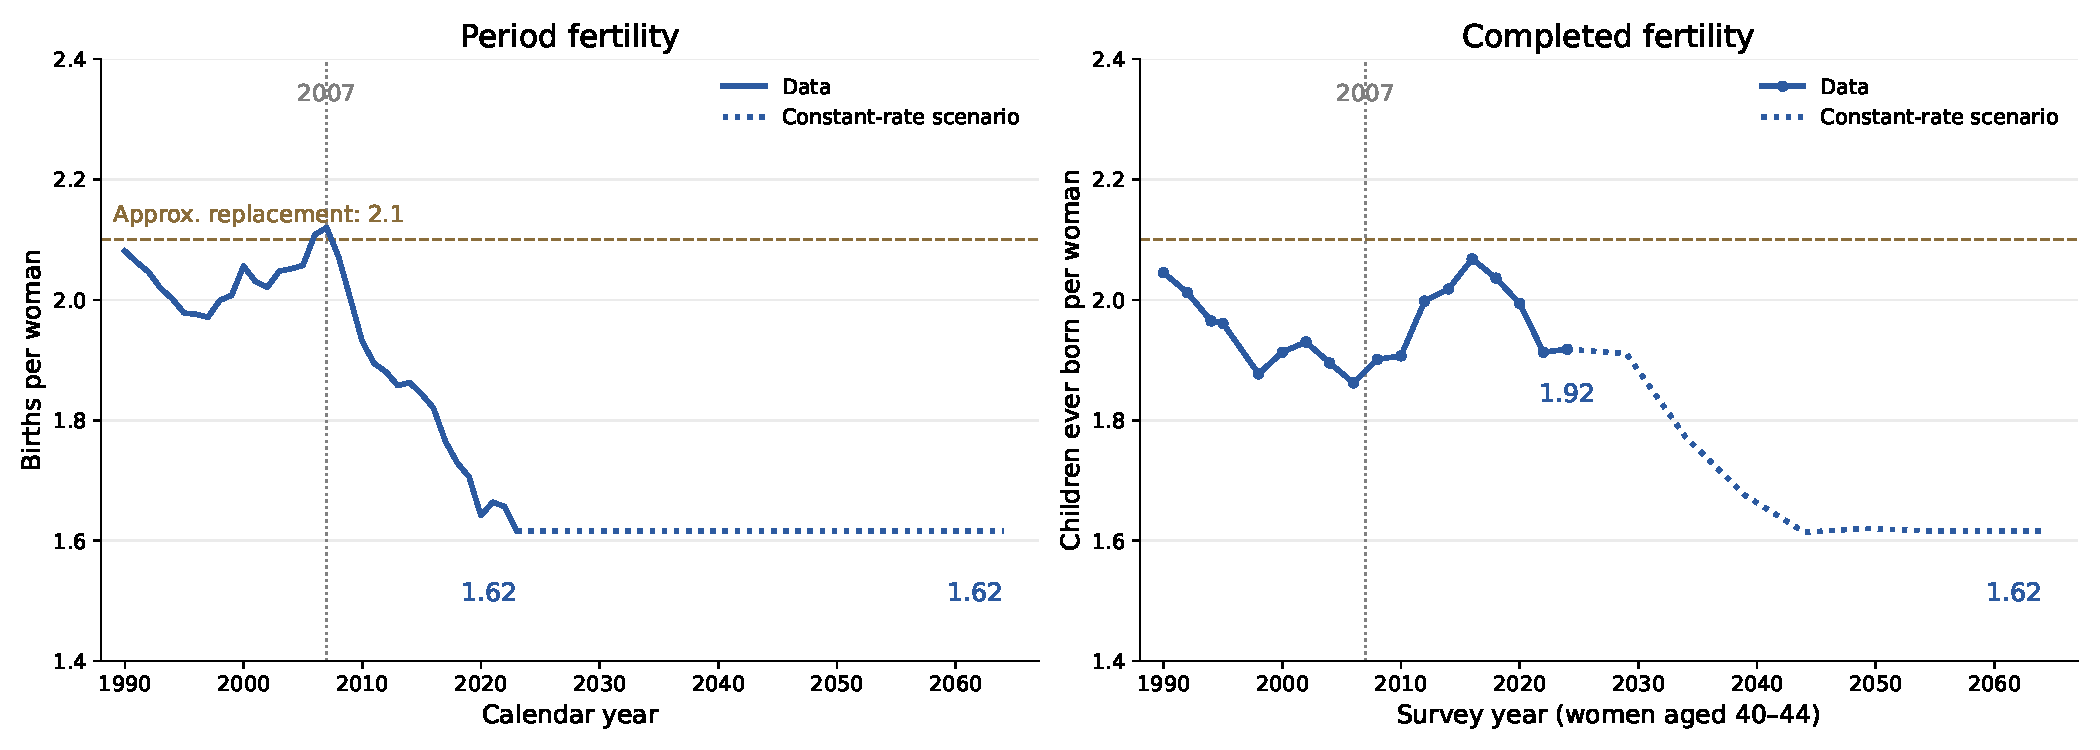
\includegraphics[width=\linewidth]{fertility_introduction_projection_1990}
\caption{Period and completed fertility in the United States}
\label{fig:quant-us-fertility}
\par\smallskip
\begin{minipage}{0.92\linewidth}
\footnotesize\textit{Notes:} Left: period total fertility rate, World
Development Indicators. Right: children ever born to women aged 40--44, CPS
Fertility Supplement. Dotted lines: a constant-rate scenario that holds period
fertility at its 2023 level; the completed-fertility continuation is rescaled
to end at that rate.
\end{minipage}
\end{figure}

Starting from the 2007 steady state, I hold all estimated parameters fixed
and let the preference for children change twice, each time unexpectedly and
believed to be permanent: from $\psi_0=0.156$ to $\psi_1=0.1311$ in 2007, and
to $\psi_2=0.110$ in 2015. The two values are chosen to match the period
fertility rate in the model's four-year periods 2011--2014 (1.861) and
2019--2022 (1.646). Between the shocks, households and the population are
carried forward, and prices, the pension and the rebate clear their markets
at every date. After 2023 the preference stays at $\psi_2$, households have
perfect foresight about prices, and the economy converges to a new stationary
equilibrium. Appendix~\ref{app:algorithms} describes the solution method.

Figure~\ref{fig:quant-transition-fit} compares the model's period fertility
with the data. The two shocks bring fertility to 1.86 in 2011--2014 and 1.65
in 2019--2022. After 2023, with the preference fixed, period fertility rises
slowly, to 1.79 by 2063. The recovery runs through the housing market: as the
smaller cohorts born after 2007 enter adulthood, the demand for rooms falls
and so does the price of space.

\begin{figure}[t]
\centering
\includegraphics[width=0.9\linewidth]{../../output/model/jmp_slides_transition_figures_20261009/fertility_fit_2007_2063.pdf}
\caption{Period fertility, model and data, 2007--2063}
\label{fig:quant-transition-fit}
\par\smallskip
\begin{minipage}{0.92\linewidth}
\footnotesize\textit{Notes:} Model: births per woman in each four-year period
of the two-shock transition from the 2007 steady state. Data: annual period
fertility and its four-year averages.
\end{minipage}
\end{figure}

Figure~\ref{fig:quant-full-transition} shows the whole transition, to 2403.
Period fertility returns to replacement after about a century and a half and
stays slightly above it for about a century before settling at replacement.
The number of households falls by about 40 percent,
to 0.594 of its 2007 level, total housing by about a quarter, and the house
price by 38 percent, to 0.485. Because the stock stays on the supply curve,
the fall in housing demand is split between a smaller stock and a lower price
in proportions set by $\eta$: with $\eta=0.63$, a stock 25 percent smaller
requires a price 38 percent lower. Along the way the price falls slowly. In 2023 it is 4.0 percent below
its 2007 steady-state level, and it is still falling in 2063.
% [MODEL] path_table_0.1311_0.110.md: benchmark price 0.7794; 2023 0.748;
% endpoint price 0.48467, population scale 0.59398, stock 4.312 vs 5.779.

\begin{figure}[t]
\centering
\includegraphics[width=\linewidth]{../../output/model/jmp_slides_transition_figures_20261009/full_transition_four_panel.pdf}
\caption{The full transition, 2007--2403}
\label{fig:quant-full-transition}
\par\smallskip
\begin{minipage}{0.92\linewidth}
\footnotesize\textit{Notes:} Period fertility, number of household heads,
total housing and the house price along the two-shock transition, with the
initial steady state normalized to 100. Diamonds mark the new stationary
equilibrium.
\end{minipage}
\end{figure}

The durability of the stock matters for this recovery.
Figure~\ref{fig:quant-full-transition-fixed} adds a path along which the
housing stock is frozen at its 2023 level. Because the rooms stay while the
population shrinks, the price falls faster and further before recovering
part of the fall, and period fertility rises above replacement from about
the 2070s, peaks near 2.2 around 2100, and settles back. The number of
households then stabilizes about 20 percent below its 2007 level rather than
40 percent. Space that cannot be withdrawn is passed on to smaller cohorts as
cheaper space, and cheaper space raises their fertility: completed fertility
of the cohort born in 2029 is 1.72 rather than 1.58, and of the cohort born
in 2057 1.93 rather than 1.72. Most of the gain is composition: fewer
households of these cohorts are still renting at ages 30 to 33, and renters
have the fewest children, although the renters who remain also gain.
% [MODEL] cohort_table.md (frozen stock vs stock that follows the price);
% "Born" in that table is the birth year of the cohort. Composition:
% notes/argument_for_corina_20261008.md step 17 (renters at 30-33 fall from
% a third to a fifth of a cohort; renters who remain 0.92 -> 1.01 for 2009).
\mocktodo{the cohort numbers come from the frozen-stock comparison of Oct 8
(cohort\_table.md); confirm they are on the same two-shock path as the
figure.}
Section~\ref{sec:policy-slow} introduces an intermediate case, a stock that
adjusts slowly toward the supply curve.

\begin{figure}[t]
\centering
\includegraphics[width=\linewidth]{../../output/model/jmp_slides_transition_figures_20261009/full_transition_four_panel_fixed.pdf}
\caption{The full transition with the housing stock fixed from 2023}
\label{fig:quant-full-transition-fixed}
\par\smallskip
\begin{minipage}{0.92\linewidth}
\footnotesize\textit{Notes:} As Figure~\ref{fig:quant-full-transition}, with
a second path (dashed) along which the housing stock is held at its 2023
level.
\end{minipage}
\end{figure}

\subsection{The 2023 economy}
\label{sec:quant-2023}

The 2023 economy is the starting point of every counterfactual, so I compare
it with the data on the same moments used in the calibration
(Table~\ref{tab:quant-2023}). None of these moments was targeted in the
transition, which matches only the period fertility rate. Housing is close to
the data: mean rooms are 5.54 against 5.58, and the room response at the first
birth and the room gap between larger and smaller families stay close to
their 2007 values in both the model and the data. Ownership among heads aged 30 to 55 is 69.6 percent against 58.7
percent: in the data ownership fell after 2007, while in the model, where
housing became cheaper, it rose. The wealth ratio is below the data, which
rose to 5.36 in 2017--2019.
\mocktodo{the 2023 wealth/earnings data value (5.36) is from the PSID 2017/19
on the narrow target definition, shown in red on the deck; confirm before
keeping it.}

\begin{table}[t]
\centering
\caption{The 2023 economy: data and model}
\label{tab:quant-2023}
\small
\begin{tabularx}{\textwidth}{@{}Xrr@{}}
\toprule
Moment & Data & Model \\
\midrule
Completed fertility, ages 40--44 & 1.92 & 1.71 \\
Childless, ages 40--44 (\%) & 18.8 & 27.4 \\
Exactly one child among mothers, 40--44 (\%) & 22.2 & 23.4 \\
Mean age at first birth (years) & 28.09 & 26.85 \\
First births at age 30+ (\%) & 37.7 & 28.2 \\
\addlinespace
Mean occupied rooms & 5.58 & 5.54 \\
Ownership, heads 30--55 (\%) & 58.7 & 69.6 \\
First-birth room response & 1.465 & 1.289 \\
Rooms: 3+ versus 1--2 resident children & 0.355 & 0.286 \\
\addlinespace
Wealth / annual gross earnings (PSID 2017/19) & 5.36 & 4.58 \\
Annual bequests / wealth (\%) & 0.88 & 0.80 \\
Wealth/income p90 / median, ages 76--84 & 3.45 & 3.31 \\
\bottomrule
\end{tabularx}
\par\smallskip
\begin{minipage}{0.95\linewidth}
\footnotesize\textit{Notes:} Model: the 2023 period of the two-shock
transition. Data: the sources of Table~\ref{tab:quant-fit} in their most
recent waves; wealth over earnings from the PSID 2017 and 2019.
\end{minipage}
\end{table}

The fertility rows are the model's largest miss, and they are informative
about what the preference shock can and cannot do. In the data, the decline
in period fertility since 2007 came with almost unchanged childlessness among
women aged 40 to 44 (19.8 percent in 2004--2006, 18.8 percent in 2024) and
with later first births: the mean age at first birth rose from 26.0 to 28.1
and the share of first births at 30 or later from 25 to 38 percent. In the
model, a lower $\psi_t$ works mainly on the extensive margin and on every
cohort alive. Women aged 40 to 44 in 2023 were 26 to 29 in 2007 and 34 to 37
in 2015, so both shocks lowered their first-birth hazard in their main
childbearing years, and 27.4 percent of them are childless. The data read the
decline as postponement among younger cohorts; the model reads it as a
permanent fall in the number of children of every cohort alive. A shock that
falls on young cohorts, or that raises the cost of early births, would bring
childlessness and the age at first birth closer to the data.
% [MODEL] childlessness_2023_miss_20261009.md.

The second miss concerns the house price. With only preference shocks,
falling fertility lowers the demand for family space, so the model has to
deliver a falling price: 4 percent below 2007 in 2023, and 10 percent below
with a slowly adjusting stock. In the data, the real house price rose by 15.6
percent between 2007 and 2023, and real rents by 15 to 19 percent. Part of the
decline in fertility since 2007 therefore came with a rising cost of space
that the estimation assigns to preferences. The transition says what housing
would have done in response to the fertility decline, not that housing caused
it.
% [DATA] Case-Shiller CSUSHPINSA / CPIAUCSL, 2023/2007 = 1.156
% (historical_supply_comparison.csv); CPI rent of primary residence, FRED.
\mocktodo{a refit with a housing-supply shock that targets the 2023 real price
as a third moment would turn this into a housing result
(housing\_tenure\_claims\_20261009.md, section 4).}

Figure~\ref{fig:quant-lifecycle-2023} compares life-cycle profiles in 2023.
The model reproduces the hump in housing size and the rise of ownership with
age, but its households buy too early, at the start of adult life, and keep
buying into old age: 40 percent of heads in their early twenties own in the
model against about 10 percent in the data, and almost all of the oldest heads
own against three quarters. Housing size peaks too early and falls too much
after 60, and children stay at home longer than in the data, because each
child leaves with a constant probability.
% [REVIEW Oct 10] lifecycle_2023.pdf and the deck do not state these numbers
% (40 percent, about 10 percent, three quarters); the figure file was not
% available to the review, so they are taken from the draft unverified.

\begin{figure}[t]
\centering
\includegraphics[width=\linewidth,trim=0 25 0 0,clip]{../../output/model/profile_2023_base14402/lifecycle_2023.pdf}
\caption{Life-cycle profiles in 2023, model and ACS}
\label{fig:quant-lifecycle-2023}
\par\smallskip
\begin{minipage}{0.92\linewidth}
\footnotesize\textit{Notes:} Homeownership, rooms and the share of households
with children at home by age of the household head. Model: the 2023 period of
the two-shock transition. Data: ACS 2023.
\end{minipage}
\end{figure}

Figure~\ref{fig:quant-allocation} returns to the allocation of large homes
documented in Section~\ref{sec:empirical-evidence}. The model reproduces the
shares held by young households without children and by middle-aged
households with children, but it gives young families with children twice
their share in the data (22.5 against 10.6 percent) and older households
without children half of theirs (21.6 against 40.0 percent). Part of the gap
is mechanical: in the model 9.3 percent of the large homes belong to old
households with a child at home, against 0.7 percent in the data, because a
child leaves with a constant probability. The model therefore understates the
intergenerational concentration of large homes. Any reallocation of space
from old to young that it predicts starts from a distribution in which the
young already hold more than they do in the data.
% [REVIEW Oct 10] 22.5 vs 10.6 and 21.6 vs 40.0 confirmed in
% notes/argument_for_corina_20261008.md (step 17 flag); 9.3 vs 0.7 not found
% in the notes and the figure file was not available to the review.

\begin{figure}[t]
\centering
\includegraphics[width=0.85\linewidth]{../../output/model/profile_2023_base14402/intergenerational_allocation_2023.pdf}
\caption{Who holds the large owner-occupied homes, model and data, 2023}
\label{fig:quant-allocation}
\par\smallskip
\begin{minipage}{0.92\linewidth}
\footnotesize\textit{Notes:} Share of owner-occupied homes with six or more
rooms held by each group, defined by the age of the householder and whether
a child lives in the home. Data: ACS 2023, as in
Figure~\ref{fig:large-homes}. Model: the 2023 period of the two-shock
transition.
\end{minipage}
\end{figure}

% ============================================================================
% October 9, 2026 build (agent draft). Replaces 05b_results.tex (Oct 6, base
% 15.07), whose numbers predate the 14.402 base and are not carried over.
% Sources, all at the 14.402 base, no new solves:
%   policy functions: output/model/jmp_slides_policy_functions_20261007/
%     child_policy.pdf, income_risk_policy.pdf (saved solution);
%   cost of a first child: latex/JMP_slides/frames/cost_of_a_first_child.pdf;
%   income risk at 2007: rental_menu_precaution_20261007/tables_price_tests.md;
%   2023 fixed-price battery: output/model/fixed_price_2023_battery_20261009/
%     (RESULTS.md, tables_2023_credit.md, bars_2023/loan_vs_insurance_bars.pdf);
%   mortgage credit and starter homes: deck frame
%     frame_mortgage_credit_starter_homes.tex and its sources;
%   PSID starter-home empirics: notes/starter_home_trap_empirics_20261009.md;
%   ranking of claims: notes/housing_tenure_claims_20261009.md.
% ============================================================================
\providecommand{\mocktodo}[1]{\textcolor{red}{[TODO: #1]}}

\section{Space, Credit and the Timing of Births}
\label{sec:results}

This section uses the calibrated model to ask which features of housing
shape fertility. I first describe how a household's choices change when a
first child arrives, and why the cost of the space a child requires bears
most heavily on households without savings. I then change, one at a time,
the price of space, access to credit, and household resources in the 2023
economy, holding prices fixed, and compare their effects on births. The
results organize around one distinction. Changes in the per-period cost of
the space a child requires, or in the buffer a household holds against that
cost, change how many children are born. Changes in the one-time cost of
getting into space, such as the down payment, change when households buy and
when they have children, and leave completed fertility within about one
percent.

\subsection{Household choices at the first birth}
\label{sec:results-policy-functions}

Figure~\ref{fig:results-policy} shows the choices of a childless renter aged
26 to 29 with middle earnings, as a function of its liquid wealth, in the
period in which it has no child and in the period in which a first child has
just been born. Without savings, the child pushes the household to the
largest rental unit, six rooms, and delays buying. With savings, the household
buys a larger home when the child arrives. Consumption falls when the child
arrives at every level of wealth. The value of trying for a child is negative
near the borrowing limit and turns positive with a small buffer, which is why
the probability of trying rises steeply with wealth at low wealth and is flat
above it.

\begin{figure}[t]
\centering
\includegraphics[width=0.85\linewidth]{../../output/model/jmp_slides_policy_functions_20261007/child_policy.pdf}
\caption{Choices with and without a first child}
\label{fig:results-policy}
\par\smallskip
\begin{minipage}{0.92\linewidth}
\footnotesize\textit{Notes:} Childless renter, age 26--29, middle earnings
state, 2007 steady state. Rooms, consumption, the probability of trying for a
child and the value of trying, by liquid wealth, in the period with no child
and with a first child just born.
\end{minipage}
\end{figure}

Figure~\ref{fig:results-cost} measures the housing cost of a first child for
childless renters of the same age without savings, at each level of earnings.
A first child raises the space the household occupies by up to two rooms.
Because renters cannot borrow, the extra rent is paid out of current income,
and at the lowest earnings consumption falls by 31 percent. The housing cost
of a child is therefore not a cost paid once but a commitment to a flow of
rent for as long as the child is at home, and it is largest relative to
income for the households that are least able to smooth it.
% [MODEL] budget_table_b0_age26_29.json (build_mechanism_readouts.py).

\begin{figure}[t]
\centering
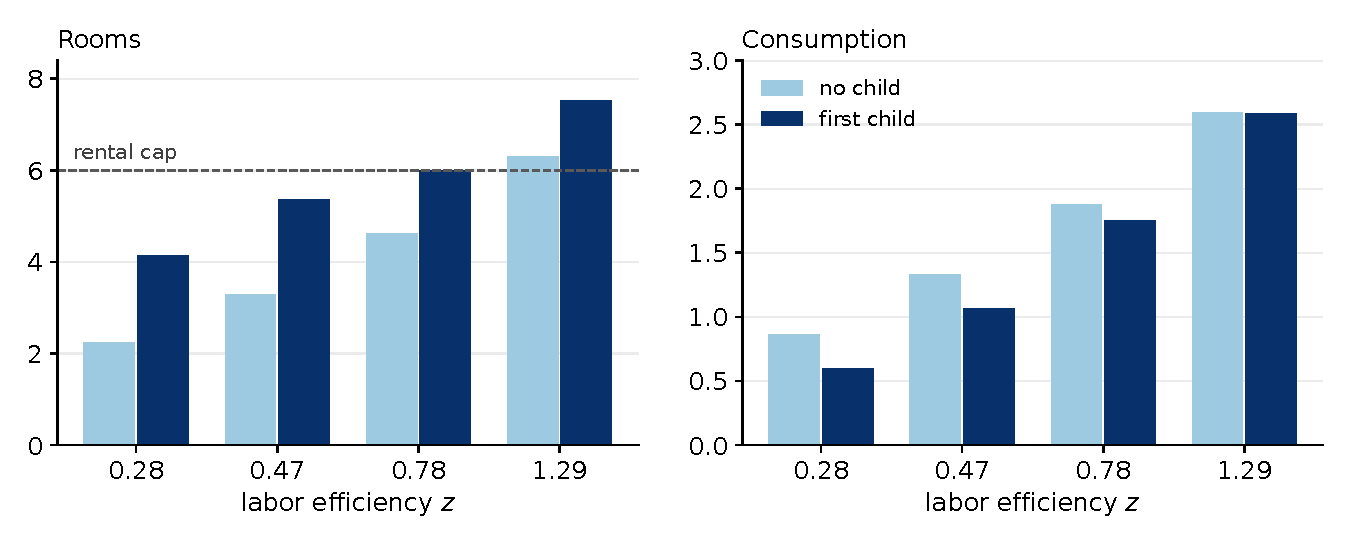
\includegraphics[width=0.85\linewidth]{../JMP_slides/frames/cost_of_a_first_child.pdf}
\caption{The housing cost of a first child}
\label{fig:results-cost}
\par\smallskip
\begin{minipage}{0.92\linewidth}
\footnotesize\textit{Notes:} Childless renters, age 26--29, no savings, by
labor efficiency $z$: rooms and consumption this period without and with a
first child. Rooms and consumption are averages over the tenure choice.
\end{minipage}
\end{figure}

A commitment to a flow of rent makes earnings risk a deterrent to
parenthood. Figure~\ref{fig:results-risk} lowers the standard deviation of
earnings innovations from 0.48 to 0.35 and plots the probability of a first
birth of a childless renter aged 26 to 29 with middle earnings. Without
savings, the probability rises from 0.41 to 0.58. With a buffer the two
curves meet: risk deters births mainly among households without savings.
Across all households, at the 2007 prices, completed fertility rises by 19
percent and childlessness falls from 19.0 to 7.4 percent. The effect of risk
grows with the commitment: in matched states, halving the variance of
earnings innovations raises first-birth attempts at ages 22 to 33 by 27.5,
38.7 and 51.1 percent with the space requirement at 80, 100 and 120 percent
of its calibrated value.
% [MODEL] completed 1.866 -> 2.220, childless 0.190 -> 0.074 (cells A6 vs
% A6_riskA); round4_tables_commitment_hazard_decomposition.md; the attempt
% numbers are confirmed in notes/housing_tenure_claims_20261009.md (claim 4).
\mocktodo{the risk experiment is large and its levels are not certified on a
clean risk solve; report a range, and rerun the floor-versus-one-time-cost
comparison at the production point to separate a commitment from a cost. The
baseline cell has completed fertility 1.866, not the calibrated 2.10, so
these cells are fixed-price cells, not the production steady state.}

\begin{figure}[t]
\centering
\includegraphics[width=0.6\linewidth]{../../output/model/jmp_slides_policy_functions_20261007/income_risk_policy.pdf}
\caption{Income risk and the probability of a first birth}
\label{fig:results-risk}
\par\smallskip
\begin{minipage}{0.92\linewidth}
\footnotesize\textit{Notes:} First-birth probability of a childless renter,
age 26--29, middle earnings, by liquid wealth, with the standard deviation of
four-year earnings innovations at its calibrated value, 0.48, and at 0.35.
Prices fixed at the 2007 steady state.
\end{minipage}
\end{figure}

\subsection{Credit, transfers and the price of space in 2023}
\label{sec:results-2023}

I now start from the 2023 economy of Section~\ref{sec:quant-2023} and make
one permanent, unanticipated change at a time. House prices, rents, the
pension and the rebate stay on their baseline paths, so each experiment
isolates the household response; any outlay is unfunded. I measure births in
2023 and completed fertility of the households aged 18 to 21 in 2023, their
mean number of children ever born at ages 46 to 49. Figure~\ref{fig:results-bars}
and Table~\ref{tab:results-2023} report the results.

\begin{figure}[t]
\centering
\includegraphics[width=\linewidth]{../../output/model/fixed_price_2023_battery_20261009/bars_2023/loan_vs_insurance_bars.pdf}
\caption{Credit, transfers and the price of space in 2023}
\label{fig:results-bars}
\par\smallskip
\begin{minipage}{0.92\linewidth}
\footnotesize\textit{Notes:} Change in completed fertility of the cohort
aged 18--21 in 2023 (left) and in its ownership at ages 18--29 (right),
relative to the baseline path. House prices and rents held on the baseline
path; one policy per row.
\end{minipage}
\end{figure}

\begin{table}[t]
\centering
\caption{Responses to housing costs, credit and transfers, 2023}
\label{tab:results-2023}
\small
\begin{tabular}{lrrr}
\toprule
 & Births, 2023 (\%) & Completed fertility (\%) & Ownership 18--29 (pp) \\
\midrule
House prices and rents $-10\%$ & $+4.7$ & $+7.0$ & $+2.5$ \\
Financed share $80\%\to95\%$ & $+0.8$ & $-1.0$ & $+25.7$ \\
Renter credit, 1 year of earnings & $+4.0$ & $+0.5$ & $-10.2$ \\
Renter credit, 2 years of earnings & $+5.8$ & $-0.8$ & $-13.5$ \\
Same total cost, paid to everyone & $+8.1$ & $+8.2$ & $+0.4$ \\
Lower income risk & $+24.2$ & $+23.6$ & $-0.1$ \\
\bottomrule
\end{tabular}
\par\smallskip
\begin{minipage}{0.92\linewidth}
\footnotesize\textit{Notes:} Changes relative to the baseline two-shock path
from 2023. Completed fertility: mean children ever born at 46--49 of
households aged 18--21 in 2023, three or more top-coded at three. Renter
credit allows renters to borrow up to one or two years of median earnings at
age 22. The transfer pays every household 0.097 per period, 3.3 percent of
mean income, the same total cost as the two-year renter credit. Lower income
risk: as in Figure~\ref{fig:results-risk}.
\mocktodo{the transfer paid only when earnings are low is pending; at 2007 it
raises completed fertility by 14.7 percent.}
\end{minipage}
\end{table}

Lower prices of space raise fertility substantially. With house prices and
rents 10 percent lower, completed fertility rises by 7.0 percent, about as
much as an unfunded transfer to every household worth 3.3 percent of mean
income (8.2 percent). Ownership of the young barely moves. The two
experiments act on the same margin: a lower rent of a room lowers the flow
cost of the space requirement, and a transfer raises the resources out of
which it is paid. The response to cash, about 2.5 percent more completed
fertility per percent of income, is of the same order as the
quasi-experimental estimates of the effect of child benefits.

Credit moves the timing of births, not their number. Raising the financed
share from 80 to 95 percent raises ownership of the young by 26 percentage
points, raises births in 2023 by 0.8 percent, and lowers completed fertility
by 1.0 percent. Credit to renters, which lets them borrow against future
earnings, raises births on impact by 4 to 6 percent and leaves completed
fertility within one percent of the baseline, consistent with households that
were waiting for a buffer having their children sooner. Both forms of credit change the
one-time cost of getting into space, the equity a buyer must hold or the
wealth a renter needs before a child, and neither changes the per-period
rent of a room, which equals the owner's user cost and does not depend on
the loan-to-value ratio. In the model, a mortgage lets a household own its
rooms sooner; it does not make those rooms cheaper to occupy.

The same distinction appears within the house price. Raising the price by
10 percent at an unchanged rent, starting from 2007, raises births on impact
by 1.1 percent and leaves completed fertility unchanged ($-0.02$ percent),
while raising both the price and the rent lowers births by 4.4 percent and
completed fertility by 5.3 percent. The response to the price at a given rent
comes from leveraged owners: births of owners whose equity is at most a
quarter of the value of their home rise by 5.0 percent, while those of
renters without savings fall by 0.1 percent. It is a change in timing.
% [MODEL] tables_capitalization.md (2007 state, rebate held); numbers
% confirmed in notes/housing_tenure_claims_20261009.md and
% notes/ptax_vs_credit_channels_20261009.md (section 2).

\subsection{Mortgage credit and starter homes}
\label{sec:results-starter}

Why does mortgage credit lower completed fertility at all, rather than leave
it unchanged? In the model, the households that credit brings into ownership
are young, childless and poor, and many of them buy the smallest home, two
rooms, which is below the space requirement and yields a parent essentially no
housing services. A household in such a home must move, and pay 6 percent of
the value to sell, before it can have a child. Table~\ref{tab:results-starter}
shows that this accounts for the effect. When the two- and four-room homes are
removed from the menu of homes for sale, the same increase in the financed
share raises ownership of the young by 4 points instead of 25, births in the
first period by 0.1 percent, and leaves completed fertility unchanged. With
the actual distribution of home sizes in the United States, credit leaves
completed fertility unchanged. Credit offered only to households that already
have children raises completed fertility by 1.2 percent; the gain is small
because parents can already rent a family-sized home.

\begin{table}[t]
\centering
\caption{Mortgage credit and the menu of homes for sale}
\label{tab:results-starter}
\small
\begin{tabular}{lrrr}
\toprule
Homes for sale & Ownership 18--29 & Births, first period & Completed fertility \\
\midrule
Without 2- and 4-room homes & 36\% $\to$ 40\% & $+0.1\%$ & $-0.05\%$ \\
With 2- and 4-room homes & 44\% $\to$ 69\% & $+0.4\%$ & $-1.4\%$ \\
\bottomrule
\end{tabular}
\par\smallskip
\begin{minipage}{0.92\linewidth}
\footnotesize\textit{Notes:} Financed share from 80 to 95 percent at fixed
house prices and rents, transfer held.
\end{minipage}
\end{table}

The starter-home mechanism is a feature of the model, not of the data. In the
model, 30 percent of young childless owners live in two rooms; in the PSID, 3
percent. And the PSID does not show the trap that the mechanism would
produce. Among couples with one child, those who own a home of at most four
rooms have the same probability of a second birth within two years as owners
of larger homes, a difference of $-0.9$ percentage points (standard error
3.5) on a base of 40 percent, and they are not stuck: 19 percent move to a
larger home within two years, against 11 percent of owners of large homes.
First-time buyers in the 2003--2007 boom bought homes of the same size as
earlier buyers, relative to their family, but paid 2.24 times their income
rather than 1.77: credit went into prices, not into smaller homes. The only
small-home gap in the data is at the first birth: childless first-time buyers
of small homes are 14 percentage points less likely to have a first child
within six years (standard error 6.7), which is as consistent with selection,
couples that do not plan children buying small, as with a trap. I therefore
read the effect of mortgage credit on completed fertility as zero to within
about one percent, and not as negative.
% [DATA] PSID-SHELF 1997-2019, code/data/starter_home_trap_20261009/.

The distinction between space and timing has one exception, and it confirms
the distinction. Credit raises fertility where it is the way into
family-sized space. If the largest rental unit had four rooms rather than
six, so that a family home had to be bought, lowering the required down
payment from 50 to 10 percent would raise completed fertility by 10.8
percent and lower childlessness from 24.9 to 18.5 percent; at the calibrated
six-room limit the same change lowers completed fertility by 1.0 percent while
raising young ownership from 22 to 62 percent. This is the direction of the
postwar mortgage expansion documented by
\citet{dettlingKearneyModernMortgage2025} and of the Brazilian housing lottery
of \citet{vandoornikFazioRamadoraiSkrastinsHousingFertility2025}, in which
credit raised family size. \citet{hacamoBabiesMortgageDeregulation2021} finds
that deregulation raised the joint probability of buying and having a child,
with no response among renters. The model reproduces the renter null and the
order of magnitude of the joint outcome; its birth response is of the same
order as his aggregate figure and far below his within-state estimate, and he
reports no completed-fertility estimate.
% [REVIEW Oct 10] notes/housing_tenure_claims_20261009.md ("stop saying" the
% model matches Hacamo) and notes/argument_for_corina_20261008.md, Oct 9
% correction; four-room numbers confirmed in RESULTS.md (cap 4, LTV 50 -> 90:
% completed +10.82%, childless 24.9 -> 18.5%; cap 6: -1.03%, own 18-29 21.8
% -> 62.0%).
\mocktodo{the four-room economy is not recalibrated (fixed prices, loss 942);
present this as a comparative static at a common price, and measure the size
distribution of rentals in the 1940 and 1950 Censuses of Housing before
mapping it to the postwar period.}

% ============================================================================
% October 9, 2026 build (agent draft). Policy section, new. Sources:
%   elastic stock (the deck's "Policy Results"):
%     output/model/policy_transition_battery_20261008/h100_torch/
%     (table_h100.md, tax_vs_credit_h100.pdf), base 14.402, from the 2023 state;
%   slow stock (deck): tax_vs_credit_h100_slow_stock.pdf;
%   by supply regime (deck appendix): ptax_by_supply_regime.pdf, h16 runs
%     (table_h16-20261008T153908-0eb8.md);
%   slow-stock refit and today's arms: output/model/slow_stock_h100_20261009/
%     README.md (project copy README-20261009T203735-9f66.md), EXPERIMENTAL;
%   channel reading: notes/ptax_vs_credit_channels_20261009.md;
%   long run: \pol macros from latex/JMP_slides/prod_tables/policy.tex
%     (reconciliation_14p40_20261007, stationary GE at psi 0.110).
% ============================================================================
\providecommand{\mocktodo}[1]{\textcolor{red}{[TODO: #1]}}

\section{A Housing Policy}
\label{sec:policy}

Section~\ref{sec:quant-2023} showed that large homes sit with older
households, and Section~\ref{sec:results} that the per-period cost of space is
what moves the number of children. A natural policy question follows: can a
policy that changes who holds housing, and at what price, raise births? I
study the experiment of \citet{coven2024}. They tax housing by value and
rebate the revenue equally to all households. Older owners, who hold the most
housing, pay more than they get back, and young renters get back more than
they pay. House prices fall, and constrained young households buy sooner or
buy bigger. I run the same experiment from the 2023 economy: the property tax
rises unexpectedly and permanently from 1.06 to 2 percent of value a year, and
its revenue is rebated equally to all households at every date. I follow
prices, rents, ownership and births along the path, and compare the tax with
the mortgage credit of Section~\ref{sec:results-2023}, raising the financed
share from 80 to 95 percent, also in general equilibrium. In both cases the
preference for children stays at its 2023 value, and every change is measured
against the baseline path from the same 2023 state.

\subsection{Results with the baseline housing supply}
\label{sec:policy-baseline}

Figure~\ref{fig:policy-baseline} reports the two policies when the housing
stock moves along the supply curve at every date. The tax lowers the house
price by 6.3 percent on impact, a gap that narrows slowly over the century.
Births fall by 0.7 percent in 2023 and are 0.3 to 0.5 percent above the
baseline from the 2030s through the 2060s. Ownership of the young rises by
about 3 percentage points on impact and stays about 2 points higher through
the 2060s. The adult population is 0.4 percent larger by 2100. Mortgage
credit raises the ownership of the young by 20 to 25 percentage points
throughout and barely moves the price. Births rise by 0.6 percent on impact,
are below the baseline from the late 2020s, and are about 2 percent lower
around 2100, when the population is 0.7 percent smaller.
% [MODEL] table_h100.md, elastic arm: price -6.33 (2023) to -6.23 (2063),
% -5.35 at the last date; births -0.69, +0.01, +0.25, +0.38, +0.47, +0.48,
% +0.68 at the last date; own 18-29 +2.83, 1.87, 1.73, 2.60, 2.54, 1.95;
% adults +0.67 at the long-run endpoint. LTV: own 18-29 +19.9 then 24.7-25.2;
% births +0.56, -0.26, -0.63, -0.64, -0.32, -0.81; adults -1.09 in the long
% run. The 2100 values are read from the figure.

\begin{figure}[t]
\centering
\includegraphics[width=0.95\linewidth,trim=0 13 0 0,clip]{../../output/model/policy_transition_battery_20261008/h100_torch/tax_vs_credit_h100.pdf}
\caption{Property tax and mortgage credit from 2023}
\label{fig:policy-baseline}
\par\smallskip
\begin{minipage}{0.92\linewidth}
\footnotesize\textit{Notes:} Change relative to the baseline path from 2023
in births, the house price, ownership at ages 18--29 and the adult population.
Property tax from 1.06 to 2 percent a year with an equal rebate; mortgage
credit: financed share from 80 to 95 percent. Housing stock on the supply
curve at every date.
\end{minipage}
\end{figure}

Why is the effect of the tax so small? A tax on value raises the cost of
holding a room. When the stock can shrink within a period, builders withdraw
rooms, so the price falls by less than the tax and the rent of a room rises:
by 13.5 percent on impact and by 10 to 12 percent later. The rebate is then
largely offset by a higher rent on the space a family needs, and births rise
by less than half a percent. At fixed prices, the same tax raises rent by 19.6
percent and lowers births by 2.9 percent on impact. What makes the tax
pro-natal, to the extent it is, is the fall in the price.

\subsection{A slowly adjusting housing stock}
\label{sec:policy-slow}

Housing is durable, and the stock cannot shrink by four percent in four
years. I therefore replace the baseline supply with a stock that adjusts
slowly. Builders replace depreciated rooms each period, and build more when
prices are high:
\begin{equation}
 I_t=\delta_H\,H_0\,P_t^{\eta},\qquad H_t=(1-\delta_H)H_{t-1}+I_t .
 \label{eq:policy-slow}
\end{equation}
In a steady state $I=\delta_H H$, so $H=H_0P^{\eta}$: the long-run supply
curve, the 2007 steady state and the calibration are unchanged, and only the
speed of adjustment differs. The stock moves toward the supply curve, closing
a fraction $\delta_H$ of the gap each year. I compare it with two extremes:
the baseline, in which the stock moves to the supply curve at once, and a
stock frozen at its 2023 level.

Figure~\ref{fig:policy-slow} repeats the two experiments with the slowly
adjusting stock. The tax now lowers the price by 11 percent on impact, and
the price gap closes over the century as the stock shrinks. Births rise by
about 2.5 percent on impact and by 3.5 to 4 percent through the middle of the
century, and the adult population is 3.5 percent larger by 2100. The
ownership of the young rises by 5 points on impact and is back to the
baseline by the 2040s. Mortgage credit is almost unaffected by the speed of
supply: young ownership rises by 19 to 27 points, births rise by less than
one percent at first and fall by 1.5 percent by 2100.

\begin{figure}[t]
\centering
\includegraphics[width=0.95\linewidth]{../../output/model/policy_transition_battery_20261008/h100_torch/tax_vs_credit_h100_slow_stock.pdf}
\caption{Property tax and mortgage credit with a slowly adjusting stock}
\label{fig:policy-slow}
\par\smallskip
\begin{minipage}{0.92\linewidth}
\footnotesize\textit{Notes:} As Figure~\ref{fig:policy-baseline}, with the
housing stock following \eqref{eq:policy-slow} from 2023.
\end{minipage}
\end{figure}

Figure~\ref{fig:policy-supply} isolates the role of supply for the tax. With
the baseline supply, rooms are withdrawn, the rent of a room rises by 13
percent, and births barely move. With a slow or a fixed stock, the rooms
stay, the house price falls instead, the rent barely moves on impact, and
births rise by about 3 percent on impact, and later by 3 to 4 percent with
the slow stock and by up to 6 percent with the fixed stock. The tax is
pro-natal when the price absorbs it, and nearly neutral when supply passes it
into rents.
% [MODEL] table_h16: frozen stock, births +2.85 on impact rising to +6.0,
% price -12.86, rent -0.10; elastic rent +13.55; fixed prices rent +19.64,
% births -2.93.
\mocktodo{the legends of the policy figures label the tax 1\%$\to$2\%; the
runs raise it from 1.06 to 2 percent. Relabel the figures.}

\begin{figure}[t]
\centering
\includegraphics[width=\linewidth]{../../output/model/jmp_slides_transition_figures_20261009/ptax_by_supply_regime.pdf}
\caption{The property tax under three housing supplies}
\label{fig:policy-supply}
\par\smallskip
\begin{minipage}{0.92\linewidth}
\footnotesize\textit{Notes:} Property tax from 1.06 to 2 percent a year,
rebated, from 2023: change relative to the no-tax path in births, the house
price, rent per room and the population, with the stock on the supply curve
at every date, adjusting slowly as in \eqref{eq:policy-slow}, or fixed at its
2023 level. Sixteen-period runs.
\end{minipage}
\end{figure}

\subsection{Where the effect of the tax comes from}
\label{sec:policy-channels}

The slowly adjusting stock changes the transition of
Section~\ref{sec:quant-transition}, so I re-estimate the two preference
shocks under it, matching the same two fertility rates, and run the tax from
the 2023 state of the re-estimated path.%
\footnote{The re-estimated shocks are $\psi_1=0.1295$ and $\psi_2=0.1062$,
which match period fertility of 1.861 and 1.646 to within 0.0004. The 2023
price is 10 percent below its 2007 level.}
Table~\ref{tab:policy-channels} reports the tax under four variants, against
the no-policy path from the same state. Births are reported in 2023, as the
mean over 2031--2035, and in 2067; completed fertility is that of the cohort
aged 18 to 21 in 2023.

\begin{table}[t]
\centering
\caption{Where the effect of the property tax comes from}
\label{tab:policy-channels}
\small
\begin{tabular}{lrrrrrr}
\toprule
 & \multicolumn{3}{c}{Births (\%)} & Completed & Price & Rent per \\
\cmidrule(lr){2-4}
 & 2023 & 2031--35 & 2067 & fertility (\%) & 2023 (\%) & room 2023 (\%) \\
\midrule
\emph{Slow stock, $\eta=0.63$} &&&&&& \\
\quad Tax, rebated & $+2.4$ & $+3.3$ & $+3.4$ & $+3.9$ & $-11.1$ & $+1.6$ \\
\quad Tax, rebate held at its base path & $-2.2$ & $-1.1$ & $-4.1$ & $-0.5$ & $-15.8$ & $-5.4$ \\
\quad Financed share $80\%\to95\%$ & $+0.9$ & $+0.2$ & $-1.1$ & $-0.6$ & $+0.1$ & $+1.8$ \\
\addlinespace
\emph{Slow stock, $\eta=1.5$} &&&&&& \\
\quad Tax, rebated & $+2.0$ & $+2.4$ & $+1.3$ & $+3.0$ & $-9.8$ & $+2.7$ \\
\addlinespace
\emph{Stock on the supply curve, $\eta=1.5$} &&&&&& \\
\quad Tax, rebated & $-2.0$ & $-1.7$ & $-3.1$ & $-1.8$ & $-3.6$ & $+18.0$ \\
\quad Financed share $80\%\to95\%$ & $+0.4$ & $-0.6$ & $-1.0$ & $-1.4$ & $+0.0$ & $+1.0$ \\
\bottomrule
\end{tabular}
\par\smallskip
\begin{minipage}{0.95\linewidth}
\footnotesize\textit{Notes:} Each row: change relative to the no-policy path
from the 2023 state of the transition re-estimated under the stated supply.
Tax: property tax from 1.06 to 2 percent a year. Completed fertility: sum of
the age-specific birth rates of the cohort aged 18--21 in 2023. With $\eta=1.5$
the supply scale is renormalized so that the 2007 steady state is unchanged.
\mocktodo{these runs are experimental (Oct 9): the slow-stock rule and
$\eta=1.5$ are not part of the calibrated model, the terminal check fails near
2400, and the $\eta=1.5$ stock-on-curve row starts from the closest grid pair
rather than the exact fit. The $\eta=1.5$ slow-stock credit arm is still
running.}
\end{minipage}
\end{table}

Three results stand out. First, the rebate carries the effect. When the
rebate is held at its base path, so that the extra revenue is not returned,
the same tax lowers births by 1.1 percent in 2031--2035 and completed
fertility by 0.5 percent, even though the price falls by 16 percent and the
rent of a room falls by 5 percent. The difference between the rebated and the
held tax is 4.4 points of births. Second, the sign of the effect follows how
much of the tax reaches the rent of a room. With a slow stock, the price
absorbs the tax and the rent rises by 1.6 to 2.7 percent on impact; births
rise by 2 to 3 percent. With a stock that can shrink quickly and an elastic
supply, the price falls by only 3.6 percent, the rent rises by 18 percent, and
births fall by about 2 percent, as at fixed prices. Third, mortgage credit
raises the ownership of the young by 19 to 21 percentage points on impact and
keeps births within about one percent of the baseline at every date, and
completed fertility within 1.5 percent, under both supplies for which the
credit arm has run.

I read these results as follows. When the price absorbs the tax, the rebated
tax is a transfer to every household, paid for by a one-time capital loss on
the households that own in 2023, at an almost unchanged rent per room. The
transfer raises the buffer of the households that decide on a first child
without savings, the margin on which Section~\ref{sec:results} found births
most responsive; the price fall itself lowers the one-time cost of buying,
which in Section~\ref{sec:results-2023} moved the timing of births and not
their number. When the price does not absorb the tax, it is a tax on rooms,
partly offset by a flat rebate, and a tax on rooms is a tax on the space
children need. The durability of the stock decides which case applies, and it
also decides who gains. The cohort young at the announcement receives the
rebate at an almost unchanged rent and has 3.9 percent more children; the
cohort aged 18 to 21 in 2031 gains less, 2.8 percent, consistent with a stock
that shrinks over time and a rent that rises with it. Births are counts, so
part of their rise at later dates reflects the larger cohorts born after the
reform rather than more children per household. The burden falls on the
owners of 2023. In the model they are less concentrated among the old than in
the data, because young families hold twice their share of the large homes
(Figure~\ref{fig:quant-allocation}).
% [REVIEW Oct 10] notes/ptax_vs_credit_channels_20261009.md marks the
% buffer and timing readings as inference [I]; the cohort numbers (3.9, 2.8)
% are in notes/housing_tenure_claims_20261009.md; "the owners are mostly old"
% is contradicted by notes/argument_for_corina_20261008.md step 17 (old
% childless hold 21.6% of large homes in the model against 40% in the data).

Two qualifications matter for how far this reading goes. The tax does not
move space to young families. Rent per room does not fall in any rebated arm,
and the gain in young ownership is small and fades. What reaches young
families is income, not rooms. And it remains open whether the housing
market matters for delivering that income. A transfer of the same size
financed by a payroll tax would show whether it matters that the rebate is
funded by a tax on housing, which falls largely on retired owners and on a
capitalized price rather than on the earnings of would-be parents.
\mocktodo{the payroll-financed arm is specified
(notes/ptax\_vs\_credit\_channels\_20261009.md) and waits on approval of the
earnings-tax patch.}

\subsection{The long run}
\label{sec:policy-longrun}

Because the population replaces itself only at 2.1 children per household,
each policy returns births per household to replacement in the long run; its
lasting effects appear in the population and in prices.
Figure~\ref{fig:policy-longrun} compares stationary equilibria at the 2023
preference for children, with and without each policy, under the baseline
supply. Relative to the stationary equilibrium without it, the property tax
changes the house price by $\pol{end_ptax2.price_pct.1}$ percent, the
population by $\pol{end_ptax2.pop_pct.1}$ percent and young ownership by
$\pol{end_ptax2.own_18_29_pp.1}$ points. Mortgage credit changes young
ownership by $\pol{end_phi095.own_18_29_pp.1}$ points, the price by
$\pol{end_phi095.price_pct.1}$ percent and the population by
$\pol{end_phi095.pop_pct.1}$ percent. At fixed prices, the tax would change
births by $\pol{ptax2_fp.births_pct.1}$ percent: the price fall is what makes
it pro-natal.

\begin{figure}[t]
\centering
\includegraphics[width=\linewidth]{../../output/model/jmp_slides_policy_functions_20261007/longrun_bars.pdf}
\caption{Property tax and mortgage credit in the long run}
\label{fig:policy-longrun}
\par\smallskip
\begin{minipage}{0.92\linewidth}
\footnotesize\textit{Notes:} Stationary equilibrium at $\psi_2=0.110$ with
each policy, relative to the stationary equilibrium without it: house price,
population and ownership at ages 18--29. Baseline housing supply.
\end{minipage}
\end{figure}

% October 9, 2026 build (agent draft): conclusion following the deck's
% "Conclusion" frame, with the property-tax claim stated as the Oct 9
% rebate-held run supports it (the deck's bullet says the tax moves space
% toward young families; rent per room does not fall in any rebated arm).
\section{Conclusion}
\label{sec:conclusion}

I build a life-cycle model of fertility with realistic housing, in which
households choose when to have children, how much space to occupy, and
whether to rent or own it. Children need space, the large homes must be
bought with a down payment, and the old hold most of them. I calibrate the
model to the United States in 2007 and treat the fall in fertility since then
as the start of a transition to a smaller population, along which a durable
housing stock makes space cheaper for the smaller cohorts that follow.

Three results emerge. First, the per-period cost of the space a child
requires, and the buffer a household holds against it, set the number of
children; the down payment, credit and the house price at a given rent set
their timing. Second, mortgage credit raises the ownership of the young by
20 to 25 percentage points and leaves completed fertility within about one
percent, except where family-sized homes cannot be rented. Third, a property
tax rebated equally to all households raises births when a durable stock lets
the price absorb the tax, by 3 to 4 percent, and lowers them when supply
passes the tax into rents. Its effect runs through the rebate: it moves income,
not space, toward young families, paid for by the owners at the time of the
reform.

The analysis has limitations that future work should address. The
preference shocks that account for the decline in fertility since 2007 fall
on every cohort alive, so the model overstates childlessness and misses the
postponement of first births, and with only preference shocks it predicts a
falling house price where the data show a rising one. The model also gives
young households too many homes and the old too few large ones. A housing
shock that matches the observed rise in prices and rents, and a fertility
shock that falls on young cohorts, are the natural next steps.

\clearpage
\appendix
\section{Data and Empirical Measurement}
\label{app:empirical-data}

\subsection{Housing stock}

The stock facts use the national public-use household file of the 2023
American Housing Survey, weighted by the housing-unit weight. Tenure has three
occupied categories: owned, rented for cash, and occupied without payment of
cash rent. Shares within a tenure use all units of that tenure as the
denominator; the share of seven-plus-room homes that are rented instead uses
all occupied units of that size. It is 8.2 percent when the denominator
contains owned and cash-rented units and 8.1 percent when it also contains
units occupied without cash rent and units with unreported tenure. Bedrooms and
total rooms are different measures. I report bedrooms for comparison with
other work and rooms because rooms are the PSID and ACS outcome and the unit of
the model. Mean rooms among households with children are computed over
households with at least one child present. A cross-section of occupied homes
does not identify the units offered for rent or the choices families would
make at other prices.

\subsection{PSID first-birth event studies}

\subsubsection*{Sample.}
The PSID data are the family and individual files for 1968--2019. An
observation is a person-year in which the person is a current member of a
family unit and at least 18 years old. The year of first birth is the earliest
birth year of a biological child in the person's relationship-to-child
history, which records up to twenty children. The comparison group consists of
persons whose full history reports no children; persons with incomplete or
unknown histories are dropped. A parent enters only if the first birth
occurs no earlier than the first year in which the person is observed as an
adult in the PSID. All estimates use the PSID longitudinal individual weight
and so include only sample persons with a positive weight.

The household sample keeps women who are the reference person or spouse of a
household containing a single current family unit, and keeps one woman per
household and year, the reference person first. The sample of adults heading a
household at baseline keeps all adults, women and men, who were reference
person or spouse in the window two to three years before the first birth, and
retains all of their person-years. The complementary sample keeps adults who
were in the PSID but not reference person or spouse in that window. Each
sample uses the same comparison group, weights and entry rule.

\subsubsection*{Housing measures.}
All four housing items are taken from the official year-specific PSID family
variables and merged to the interview year in which they were reported. Rooms
are the total rooms in the dwelling. Codes that do not denote a count (9
through 1984; 99 in 1985--1993; 98 and 99 from 1994) are set to missing, and a
reported zero is retained. Ownership equals one if the family owns the
dwelling and zero if it rents; other arrangements are missing. The mobility
item asks whether the family moved since a fixed date: the spring of the
previous survey year in the annual waves, and January 1 of the previous survey
year in recent waves. It therefore records a move within an interval of about
one year in the annual waves and about two years in the biennial waves. The reason for a move is the first-mentioned
reason. ``More space'' is the PSID category for expansion of housing (more
space, more rent, a better place); ``neighborhood'' is the category for
neighborhood-related reasons (a better neighborhood, schooling, proximity to
friends or relatives). Unknown or unreported answers are missing, and code 9
of the reason item (unknown before 2019, homelessness in 2019) is treated as
missing throughout. An observation contributes to an outcome only when that
outcome is reported; unreported outcomes are never coded as zero.

A merged PSID panel used in earlier versions of this analysis stored rooms,
the mobility item and the reason for moving on the row of the interview
before the one at which they were reported, one year earlier through 1997 and
two years earlier afterwards. All 811,486 room values in that panel that
overlap the official variables equal the official value from the following
interview. An earlier estimate of 0.77 rooms three years after the birth
therefore compared rooms four to five years after the birth with rooms in the
year before or the year of the birth; the estimates in the text supersede it.

\subsubsection*{Estimator.}
Event time is the survey year minus the year of first birth, grouped into the
windows $\le-8$, $-7/{-6}$, $-5/{-4}$, $-3/{-2}$, $-1/0$, $+1/{+2}$,
$+3/{+4}$, $+5/{+6}$, $+7/{+8}$, $+9/{+10}$ and $\ge+11$. Two-year windows
are needed because the PSID became biennial after 1997: from the 1999 birth
cohort on, no cohort is observed at both single years $-2$ and $+3$, so a
single-year reference period is observed for only part of the cohorts. The
omitted window is $-3/{-2}$, and each birth cohort must be observed in it;
cohorts without an observation in the reference window are excluded (first
births in 1968--1970 and 1985--1986 in the household sample, none in the
sample fixed at baseline). I estimate cohort-specific event paths relative to
the comparison group and average them with cohort-share weights, following Sun
and Abraham (2021). The regressions include person and survey-year fixed
effects and complete sets of indicators for age and years of education.
Standard errors are clustered by person and account for the estimation of the
cohort shares.

\subsubsection*{Robustness.}
Table~\ref{tab:app-rooms-robust} collects alternative rooms estimates for the
household sample. With the year before the birth in the reference window
($-2/{-1}$), rooms are 0.76 higher two to three years after the birth. Moving
the reference window earlier raises the estimate at three to four years
because it counts the pre-birth rise in this sample; the increase measured from
years $-3/{-2}$ is 1.03, 1.00 and 0.94 across the three reference windows.
Taking rooms from the merged panel, re-dated to the
interview at which they were reported, instead of from the official variables
changes the estimate by 0.02. Using the latest birth cohort instead of the
childless as comparison group leaves it unchanged. Requiring the first birth
to follow the woman's first observation as reference person or spouse, rather
than her first observation as an adult, lowers it by 0.05 and removes 24
percent of the observations.

\begin{table}[H]
\centering
\caption{Rooms around the first birth: alternative samples and reference windows (PSID)}
\label{tab:app-rooms-robust}
\small
\begin{tabularx}{\textwidth}{@{}X l l c r@{}}
\toprule
Sample & Reference & Window & Rooms (SE) & Person-years \\
\midrule
Women reference person or spouse, each year & $-3/{-2}$ & $+3/{+4}$ & 1.03 (0.07) & 63,338 \\
\quad same & $-2/{-1}$ & $+2/{+3}$ & 0.76 (0.06) & 65,053 \\
\quad same & $-5/{-4}$ & $+3/{+4}$ & 1.30 (0.10) & 59,623 \\
\quad same & $-7/{-6}$ & $+3/{+4}$ & 1.43 (0.13) & 56,749 \\
\quad same, first birth after first year as reference person or spouse & $-3/{-2}$ & $+3/{+4}$ & 0.97 (0.07) & 48,225 \\
\addlinespace
Adults reference person or spouse in $-3/{-2}$ & $-3/{-2}$ & $+3/{+4}$ & 1.47 (0.05) & 117,853 \\
Adults not reference person or spouse in $-3/{-2}$ & $-3/{-2}$ & $+3/{+4}$ & $-0.38$ (0.08) & 87,239 \\
All adults & $-3/{-2}$ & $+3/{+4}$ & 0.97 (0.05) & 187,873 \\
\bottomrule
\end{tabularx}
\par\smallskip
\begin{minipage}{0.97\linewidth}
\footnotesize\textit{Notes:} Same estimator, comparison group, controls and
weights as Table~\ref{tab:app-rooms-path}. ``Reference'' is the omitted window
and ``Window'' the reported one, both in years relative to the first birth.
Rows with an earlier reference window measure the change from that window, so
they include the pre-birth rise of the household sample.
\end{minipage}
\end{table}

\subsection{ACS matched pseudo-panel}

The ACS exercise uses the one-year samples for 2005--2019 in all states and
the District of Columbia. The sample consists of women aged 25 to 45. Because
the ACS contains no birth histories, the year of first birth is inferred from
the age of the oldest child linked to the woman in the household roster, and a
woman's housing before that year is represented by childless women surveyed in
the corresponding earlier years who share her demographic matching cell.
Housing outcomes do not enter the matching. Rooms are capped at nine, and codes
that do not denote a count are missing; bedrooms are capped at five; ownership
equals one for owned units and zero for rented ones. The regression includes
event-time indicators from $-5$ to $+10$ with year $-2$ omitted, and state, age
and survey-year fixed effects; it is weighted by the matching weights, with
standard errors clustered by source household because a household can supply
several matched records. The estimation sample has 14.2 million matched
records from 2.8 million source households.

Between one year before and three years after the birth, rooms rise by 0.49
(0.01), bedrooms by 0.34 (0.004), and the ownership rate by 3.3 percentage
points (0.2). Dropping the age fixed effects, or all fixed effects, raises the
room estimate to 0.70 and 0.71 and the ownership estimate to 10.6 and 10.7
points; dropping the state and survey-year effects gives 0.53 rooms and 4.3
points. The pre-birth observations are constructed from other
women, so the design assumes that matched childless women represent the
housing future mothers would have had before the birth. The roster does not
record children living elsewhere or distinguish biological from other
children.

\subsection{Sibling-composition designs}

The ACS sibling designs use women aged 21 to 35 in the 2005--2019 one-year
samples whose oldest linked child, if any, is younger than 18. Children are
linked to mothers through the household roster, which records children living
with the mother, not all children borne, and does not separate biological from
step or adoptive children. The regressions control for complete sets of
indicators for the mother's age at the event, her race, the survey year and
the event age, are weighted by the person weight, and cluster standard errors
by household.

In the first design, the sample is mothers whose oldest linked child is aged 0
to 5 (857,607 mothers). The instrument indicates that the two oldest children
are recorded at the same age, and the treatment is a second resident child.
Ages are recorded in whole years without quarter of birth, so the instrument
is an age-only proxy for a twin birth. The first stage is 0.66 ($F$ statistic
above 77,000). The reduced form is 0.33 rooms (0.02), and the implied effect of
a second child is 0.50 rooms (95 percent interval 0.45 to 0.55), 0.33 bedrooms
(0.31 to 0.36), and 4.7 percentage points in ownership (3.3 to 6.1).

In the second design, the sample is mothers whose two oldest linked children
differ in age and whose second child is aged 0 to 5 (656,986 mothers); it is
not restricted to mothers with exactly two children. The instrument indicates
that the two oldest children have the same sex, and the treatment is a third
resident child. The first stage is 0.033 ($F=715$). Mothers of same-sex pairs
live in 0.038 fewer rooms (0.005) and 0.034 fewer bedrooms (0.003), and their
ownership rate does not differ. Scaled by the first stage, a third child would
reduce the dwelling by 1.15 rooms (95 percent interval 0.83 to 1.47). Children of the same sex can
share a bedroom, so sibling sex composition may change the space a family
needs without changing its size. That possibility would violate the exclusion
restriction for housing outcomes. The data cannot test it formally, and I do
not interpret this estimate as the effect of a third child. The same two designs are too imprecise in the PSID to add
information: same-age births are rare in its smaller sample, and the
sex-composition first stage is weak.

\subsection{Estimates and the second sample}
\label{app:empirical-two-samples}

Tables~\ref{tab:app-rooms-path} and \ref{tab:app-tenure-moves} report the
estimates behind Figures~\ref{fig:emp-rooms-path} and
\ref{fig:emp-tenure-moves}, for the household sample of the main text and for
a second sample that fixes household position before the birth. The second
sample keeps every adult, woman or man, who was a reference person or spouse
two to three years before the birth, and follows that person in every year.
Both partners of a couple can appear in it, so its person-clustered standard
errors are somewhat too small. Figures~\ref{fig:app-rooms-samples} and
\ref{fig:app-tenure-samples} plot the two samples together. Fixing household
position before the birth, the pre-birth path is flat; the household sample's
rise in the four years before the reference window reflects who is in the
sample at that point.

\begin{figure}[p]
\centering
\includegraphics[width=0.9\linewidth]{first_birth_rooms_psid_samples}
\caption{Rooms around the first birth, two samples (PSID)}
\label{fig:app-rooms-samples}
\end{figure}

\begin{figure}[p]
\centering
\includegraphics[width=0.95\linewidth]{first_birth_tenure_moves_psid_samples}
\caption{Ownership and moving around the first birth, two samples (PSID)}
\label{fig:app-tenure-samples}
\end{figure}

\begin{table}[p]
\centering
\caption{Rooms around the first birth (PSID)}
\label{tab:app-rooms-path}
\small
\begin{tabular}{@{}l c c@{}}
\toprule
 & Women who are reference & Adults who were reference \\
 & person or spouse & person or spouse two to \\
 & in each year & three years before the birth \\
\midrule
\multicolumn{3}{@{}l}{\textit{Years relative to first birth: change in rooms relative to years $-3$ and $-2$}} \\
$-8$ or earlier & $-0.50$ (0.12) & $\phantom{-}0.15$ (0.08) \\
$-7$ and $-6$ & $-0.50$ (0.10) & $\phantom{-}0.04$ (0.06) \\
$-5$ and $-4$ & $-0.34$ (0.06) & $-0.03$ (0.04) \\
$-3$ and $-2$ & 0 & 0 \\
$-1$ and $0$ & $\phantom{-}0.41$ (0.05) & $\phantom{-}0.61$ (0.04) \\
$+1$ and $+2$ & $\phantom{-}0.82$ (0.06) & $\phantom{-}1.19$ (0.04) \\
$+3$ and $+4$ & $\phantom{-}1.03$ (0.07) & $\phantom{-}1.47$ (0.05) \\
$+5$ and $+6$ & $\phantom{-}1.17$ (0.08) & $\phantom{-}1.62$ (0.06) \\
$+7$ and $+8$ & $\phantom{-}1.20$ (0.09) & $\phantom{-}1.64$ (0.07) \\
$+9$ and $+10$ & $\phantom{-}1.25$ (0.10) & $\phantom{-}1.83$ (0.08) \\
$+11$ or later & $\phantom{-}1.16$ (0.13) & $\phantom{-}1.85$ (0.09) \\
\midrule
Mean rooms, years $-3$ and $-2$ & 4.70 & 4.69 \\
Person-years & 63,338 & 117,853 \\
Persons: first-time parents / childless & 3,655 / 1,654 & 3,302 / 6,008 \\
\bottomrule
\end{tabular}
\par\smallskip
\begin{minipage}{0.97\linewidth}
\footnotesize\textit{Notes:} Interaction-weighted event-study estimates
(Sun and Abraham, 2021) in two-year windows of event time, with standard errors
clustered by person in parentheses. The comparison group consists of adults
with no children in their full relationship history. All regressions include
person and survey-year fixed effects and indicators for age and years of
education, and use PSID longitudinal weights. Rooms are the total rooms in the
dwelling reported at the interview. The first column excludes first births in
1968--1970 and 1985--1986, which have no observation in the reference window.
\end{minipage}
\end{table}

\begin{table}[p]
\centering
\caption{Ownership and moving around the first birth (PSID)}
\label{tab:app-tenure-moves}
\footnotesize
\setlength{\tabcolsep}{4pt}
\begin{tabular}{@{}l c c c c c r@{}}
\toprule
 & Mean, & \multicolumn{4}{c}{Change relative to years $-3$ and $-2$} & Person- \\
\cmidrule(lr){3-6}
 & $-3/{-2}$ & $-1/0$ & $+1/{+2}$ & $+3/{+4}$ & $+5/{+6}$ & years \\
\midrule
\multicolumn{7}{@{}l}{\textit{A. Women who are reference person or spouse in each year}} \\
Owns the dwelling & 0.41 & $\phantom{-}0.11$ (0.01) & $\phantom{-}0.16$ (0.02) & $\phantom{-}0.16$ (0.02) & $\phantom{-}0.14$ (0.02) & 61,229 \\
Moved since last interview & 0.58 & $-0.04$ (0.02) & $-0.12$ (0.02) & $-0.16$ (0.02) & $-0.16$ (0.02) & 63,817 \\
Moved for more space & 0.070 & $\phantom{-}0.014$ (0.009) & $\phantom{-}0.034$ (0.009) & $\phantom{-}0.020$ (0.010) & $\phantom{-}0.007$ (0.010) & 62,813 \\
Moved for neighborhood & 0.032 & $-0.004$ (0.006) & $-0.005$ (0.006) & $-0.010$ (0.005) & $\phantom{-}0.002$ (0.006) & 62,813 \\
\multicolumn{7}{@{}l}{\quad\textit{Share of moves, households that moved:}} \\
\quad Share for more space & 0.122 & $\phantom{-}0.054$ (0.017) & $\phantom{-}0.140$ (0.021) & $\phantom{-}0.133$ (0.023) & $\phantom{-}0.108$ (0.026) & 19,456 \\
\quad Share for neighborhood & 0.054 & $-0.017$ (0.012) & $-0.011$ (0.014) & $-0.017$ (0.014) & $\phantom{-}0.022$ (0.018) & 19,456 \\
\addlinespace
\multicolumn{7}{@{}l}{\textit{B. Adults who were reference person or spouse two to three years before the birth}} \\
Owns the dwelling & 0.43 & $\phantom{-}0.16$ (0.01) & $\phantom{-}0.25$ (0.01) & $\phantom{-}0.27$ (0.01) & $\phantom{-}0.26$ (0.01) & 111,272 \\
Moved since last interview & 0.54 & $-0.08$ (0.01) & $-0.17$ (0.01) & $-0.21$ (0.01) & $-0.21$ (0.01) & 118,875 \\
Moved for more space & 0.064 & $\phantom{-}0.015$ (0.006) & $\phantom{-}0.021$ (0.006) & $\phantom{-}0.010$ (0.006) & $\phantom{-}0.009$ (0.006) & 116,697 \\
Moved for neighborhood & 0.030 & $-0.009$ (0.004) & $-0.008$ (0.004) & $-0.009$ (0.004) & $-0.003$ (0.004) & 116,697 \\
\multicolumn{7}{@{}l}{\quad\textit{Share of moves, households that moved:}} \\
\quad Share for more space & 0.123 & $\phantom{-}0.050$ (0.013) & $\phantom{-}0.114$ (0.017) & $\phantom{-}0.142$ (0.020) & $\phantom{-}0.147$ (0.022) & 27,462 \\
\quad Share for neighborhood & 0.058 & $-0.022$ (0.009) & $\phantom{-}0.005$ (0.011) & $-0.002$ (0.013) & $\phantom{-}0.012$ (0.015) & 27,462 \\
\bottomrule
\end{tabular}
\par\smallskip
\begin{minipage}{0.97\linewidth}
\footnotesize\textit{Notes:} Same estimator, comparison group, controls,
weights and reference window as Table~\ref{tab:app-rooms-path}. Columns are
windows of years relative to the first birth. Entries are changes relative to
years $-3$ and $-2$, with person-clustered standard errors
in parentheses; the first column is the weighted mean in the reference window.
Each outcome uses its own sample of non-missing observations. ``Moved for more
space'' equals one if the household moved since the previous interview and
gave expansion of housing (more space, a better place) as the first reason,
and zero otherwise; ``moved for neighborhood'' is defined in the same way. The
rows for households that moved restrict the sample to household-years with a
move and therefore condition on an outcome of the birth.
\end{minipage}
\end{table}

% October 9, 2026 build (agent draft): model appendices following the deck's
% appendix (supply arms, CES variant, solution algorithms). Tables for the CES
% variant are the deck's generated files (latex/JMP_slides/ces_tables/).
\section{Housing Supply Arms}
\label{app:supply}

Figure~\ref{fig:app-slow-transition} compares the estimated transition of
Section~\ref{sec:quant-transition}, in which the stock stays on the supply
curve, with the same path when the stock adjusts slowly from 2023, as in
\eqref{eq:policy-slow}. With the slow stock, households fall less in the
first century, total housing falls more slowly, and the price falls faster at
first; the two paths reach the same stationary equilibrium.
Figures~\ref{fig:app-slow-policies} and~\ref{fig:app-frozen-policies} show the
paths of the policies of Section~\ref{sec:policy} with the slowly adjusting
and the frozen stock.
\mocktodo{the deck's own note: refit the 2007--2023 transition under the
slowly adjusting stock for these figures (the re-estimated pair of
Table~\ref{tab:policy-channels} exists for the tax arms only).}

\begin{figure}[p]
\centering
\includegraphics[width=\linewidth,trim=0 0 0 50,clip]{../../output/model/transition_h100_14402_20261007/appendix_supply_arms_20261009/slow_stock_vs_estimated.pdf}
\caption{Estimated transition and a slowly adjusting stock from 2023}
\label{fig:app-slow-transition}
\end{figure}

\begin{figure}[p]
\centering
\includegraphics[width=\linewidth,trim=0 0 0 50,clip]{../../output/model/transition_h100_14402_20261007/appendix_supply_arms_20261009/slow_stock_policies.pdf}
\caption{Policies from 2023 with a slowly adjusting stock}
\label{fig:app-slow-policies}
\par\medskip
\includegraphics[width=\linewidth,trim=0 0 0 50,clip]{../../output/model/transition_h100_14402_20261007/appendix_supply_arms_20261009/frozen_stock_policies.pdf}
\caption{Policies from 2023 with the stock frozen at its 2023 level}
\label{fig:app-frozen-policies}
\end{figure}

\section{A CES Housing Composite}
\label{app:ces}

The baseline combines a Cobb--Douglas composite with the space requirement
$h_P$. As a robustness check I replace both with a CES composite in which
children raise the rooms needed for given housing services:
\begin{equation}
 u_t=\frac{1}{1-\sigma}\left(\frac{Q_t}{e(m_t)}\right)^{1-\sigma}+\psi_t m_t^{1-\gamma},\qquad
 Q_t=\Bigl[\alpha_0\,c_t^{\rho}+(1-\alpha_0)\Bigl(\frac{\chi^{\1\{\mathrm{own}\}}\,h_t}{k(m_t)}\Bigr)^{\rho}\Bigr]^{1/\rho},
\end{equation}
with $\rho=(\varepsilon-1)/\varepsilon$, $\varepsilon=0.67$, and
$k(m_t)=\exp\bigl[\eta_1\1\{m_t\ge1\}+\eta_2\max(m_t-1,0)\bigr]$. Housing and
consumption are complements, and without a floor space is not a fixed entry
cost of a child. I estimate $\eta_1$ and $\eta_2$, the rooms needed by the
first and each later child at home, and $\alpha_0$, so twelve parameters are
chosen to match thirteen moments. The new moments are the rent share of
renters aged 30--55 with no child at home (0.360, CE), the probability of
moving from renting to owning within four years at ages 22--41 (0.281, PSID),
and the share of mothers with three or more children (0.357, CPS). The rooms
added at the first birth are re-measured (1.025, PSID), the room gap between
larger and smaller families becomes a target, and the recent-parent
ownership gap becomes a validation moment.

% completed fertility at 46--49, CES at the calibrated point, fixed price and rebate (generated)
\def\cesLTVhundred{$+0.1\%$}
\def\cesLowerRisk{$+13.2\%$}
\def\cesCapTen{$+0.5\%$}

Table~\ref{tab:app-ces-fit} reports the fit. It is worse than the
benchmark's: slightly better on childlessness, family size, rooms and the
rooms at first birth, and worse on timing, ownership, the rent share, the
family room gap, wealth and bequests. The responses of completed fertility
are as in the benchmark: \cesLTVhundred{} with 100 percent financing,
\cesLowerRisk{} with lower earnings risk, and \cesCapTen{} with a ten-room
rental cap.

\begin{table}[t]
\centering
\caption{CES variant: targets and fit}
\label{tab:app-ces-fit}
\small
\begin{minipage}[t]{0.66\linewidth}\vspace{0pt}
\begin{tabularx}{\textwidth}{@{}Xrrr@{}}
\toprule
Moment & Target & CES & Cobb--Douglas \\
\midrule
Childless, women 40--44 (\%) & 19.8 & 20.1 & 20.2 \\
One child among mothers, 40--44 (\%) & 21.4 & 21.5 & 21.7 \\
Mothers with 3+ children, 40--44 (\%) & 35.7 & 38.7 & 39.5 \\
Mean age at first birth (years) & 25.98 & 26.02 & 25.96 \\
Children ever born by age 25 & 0.810 & 0.542 & 0.553 \\
\addlinespace[3pt]
Mean occupied rooms & 5.73 & 5.80 & 5.82 \\
Ownership, heads 30--55 (\%) & 67.6 & 66.6 & 67.0 \\
Renter to owner within 4 years (\%) & 28.1 & 34.7 & 31.0 \\
Rent share, childless renters (\%) & 36.0 & 17.2 & 23.3 \\
First-birth room response & 1.025 & 0.801 & 1.264 \\
Room gap, 3+ vs 1--2 children at home & 0.385 & 0.538 & 0.294 \\
\addlinespace[3pt]
Wealth / annual gross earnings & 4.46 & 5.07 & 4.58 \\
Annual bequests / wealth (\%) & 0.73 & 0.86 & 0.71 \\
\bottomrule
\end{tabularx}

\end{minipage}\hfill
\begin{minipage}[t]{0.3\linewidth}\vspace{0pt}
\begin{tabular}{@{}lr@{}}
\toprule
Parameter & Value \\
\midrule
$\beta_{\rm annual}$ & 0.948 \\ % Annual discount factor
$\kappa_1$ & 0.100 \\ % First-birth taste scale
$\kappa_C$ & 0.246 \\ % Later-birth taste scale
$\chi$ & 1.061 \\ % Owner housing-service multiplier
$H_0$ & 7.941 \\ % Housing supply scale
$\theta_0$ & 0.421 \\ % Bequest-motive scale
$\xi$ & 0.304 \\ % First-birth utility cost
$\psi_0$ & 0.150 \\ % Initial preference for children
$\gamma$ & 0.156 \\ % Curvature of the benefit of children
$\kappa_T$ & 0.016 \\ % Tenure taste scale
$\alpha_0$ & 0.720 \\ % Consumption weight in the composite
$\eta_1$ & 0.630 \\ % Housing need of the first child
$\eta_2$ & 0.059 \\ % Housing need of each later child
\bottomrule
\end{tabular}

\end{minipage}
\end{table}

Before recalibration, Table~\ref{tab:app-ces-credit} re-fits only $\psi$ to
19 percent childlessness under each specification, at fixed prices and the
six-room rental cap. Mortgage credit moves completed fertility by between $-2$
and $+0.3$ percent in all thirteen specifications that reach 19 percent
childlessness, and the negative sign comes mostly from the floor. Credit to
renters raises births on impact by 6 to 9 percent and completed fertility by
between $-0.6$ and $+2.4$ percent in the cases shown.

\begin{table}[t]
\centering
\caption{CES variant: credit across specifications}
\label{tab:app-ces-credit}
\small\setlength{\tabcolsep}{4pt}
\begin{tabularx}{\textwidth}{@{}Xccc rr rr@{}}
\toprule
 & & & & \multicolumn{2}{c}{Financed share $80\%\to95\%$} & \multicolumn{2}{c}{Renter credit, 2 years} \\
\cmidrule(lr){5-6}\cmidrule(l){7-8}
 & $\varepsilon$ & Floor & Need $k$ & Impact & Completed & Impact & Completed \\
\midrule
Cobb--Douglas (benchmark) & 1 & yes & 1 & $+0.42\%$ & $-1.35\%$ & $+8.5\%$ & $+0.62\%$ \\
CES & 0.5 & yes & 1 & $-0.16\%$ & $-1.40\%$ & $+8.0\%$ & $+0.22\%$ \\
CES & 0.25 & yes & 1 & $-0.06\%$ & $-0.87\%$ & $+7.3\%$ & $-0.25\%$ \\
CES & 0.5 & yes & 1.5 & $+0.05\%$ & $-1.10\%$ & $+7.0\%$ & $-0.63\%$ \\
CES, no floor & 0.5 & no & 1 & $+0.44\%$ & $-0.03\%$ & $+6.9\%$ & $+2.25\%$ \\
CES, no floor & 0.5 & no & 1.5 & $+0.51\%$ & $-0.18\%$ & $+8.3\%$ & $+2.39\%$ \\
Cobb--Douglas, no floor & 1 & no & 1.5 & $+1.03\%$ & $+0.23\%$ & $+8.3\%$ & $+2.42\%$ \\
\bottomrule
\end{tabularx}
\par\smallskip
\begin{minipage}{0.95\linewidth}
\footnotesize\textit{Notes:} Each row re-fits only $\psi$ to 19 percent
childlessness; house prices fixed, rental cap of six rooms.
\end{minipage}
\end{table}

\section{Solution Algorithms}
\label{app:algorithms}

\paragraph{Stationary equilibrium.} I solve for the house price $P$, the
pension $\varpi$ and the rebate $T$, given parameters and a fixed preference
for children.
\begin{enumerate}
\item Guess $(P,\varpi,T)$ and derive the rent $r$ from the user cost.
\item Solve the household problem backward over age and compute the choice
probabilities.
\item Construct the stationary distribution of households. Set the mass of
households equal to housing supply divided by mean housing per household.
\item Compute three residuals: excess demand for housing, the pension budget
and the rebate budget. The loss is the largest residual in absolute value.
\item Update $(P,\varpi,T)$ and repeat until the loss is below tolerance.
Then apply the population law for one period and verify that the
distribution reproduces itself.
\end{enumerate}

\paragraph{Transition.} I solve for the paths $(P_t,\varpi_t,T_t)_{t\geq t_0}$,
given the inherited households and a preference believed permanent.
\begin{enumerate}
\item Solve the new stationary equilibrium; it supplies the terminal value
function.
\item Guess the three paths and derive rents from \eqref{eq:m-rent}.
\item Solve the household problem backward in calendar time from the terminal
value.
\item Advance households and the queue of entrants forward from the inherited
state, and aggregate housing demand and taxes at each date.
\item Compute the three residuals at every date. The loss is the largest
residual across dates.
\item Update the paths jointly and repeat until the loss is below tolerance.
Extend the horizon to check that early responses are stable.
\end{enumerate}
The transitions in the paper use 100 four-year periods, with tolerances of
$2\times10^{-4}$ on the housing market and $2\times10^{-5}$ on the pension and
the rebate.


\clearpage
\bibliographystyle{plainnat}
\bibliography{../references,../main_bib,../lit_review_extra}

\end{document}
